%!TEX root = ../dissertation.tex
\begin{savequote}[75mm]
A picture is worth a thousand swords.
\qauthor{Tony}
\end{savequote}

\chapter{Reconstruction and Objects}

%%%%%%%%%%%%%%
\paragraph{}
Reconstruction is the construction of particles from raw detector readouts. 
In each $pp$ collision recorded by ATLAS, charged particles bend in the magnetic field and leave tracks in the ID, electrons and photons deposit their energies in ECAL, hadrons are absorbed in HCAL, muons leave extra tracks in the MS, and neutrinos are inferred by the conservation of momentum in the transverse plane. 
Figure~\ref{fig:obj_reco_overview} gives an overview of the different sub-detectors that each type of particle will interact with in ATLAS. Quark reconstruction and identification is particularly important for this thesis, with di-Higgs decaying to \bbbb.

\begin{figure}[htbp!]
  \centering
  \captionsetup{justification=centering}
  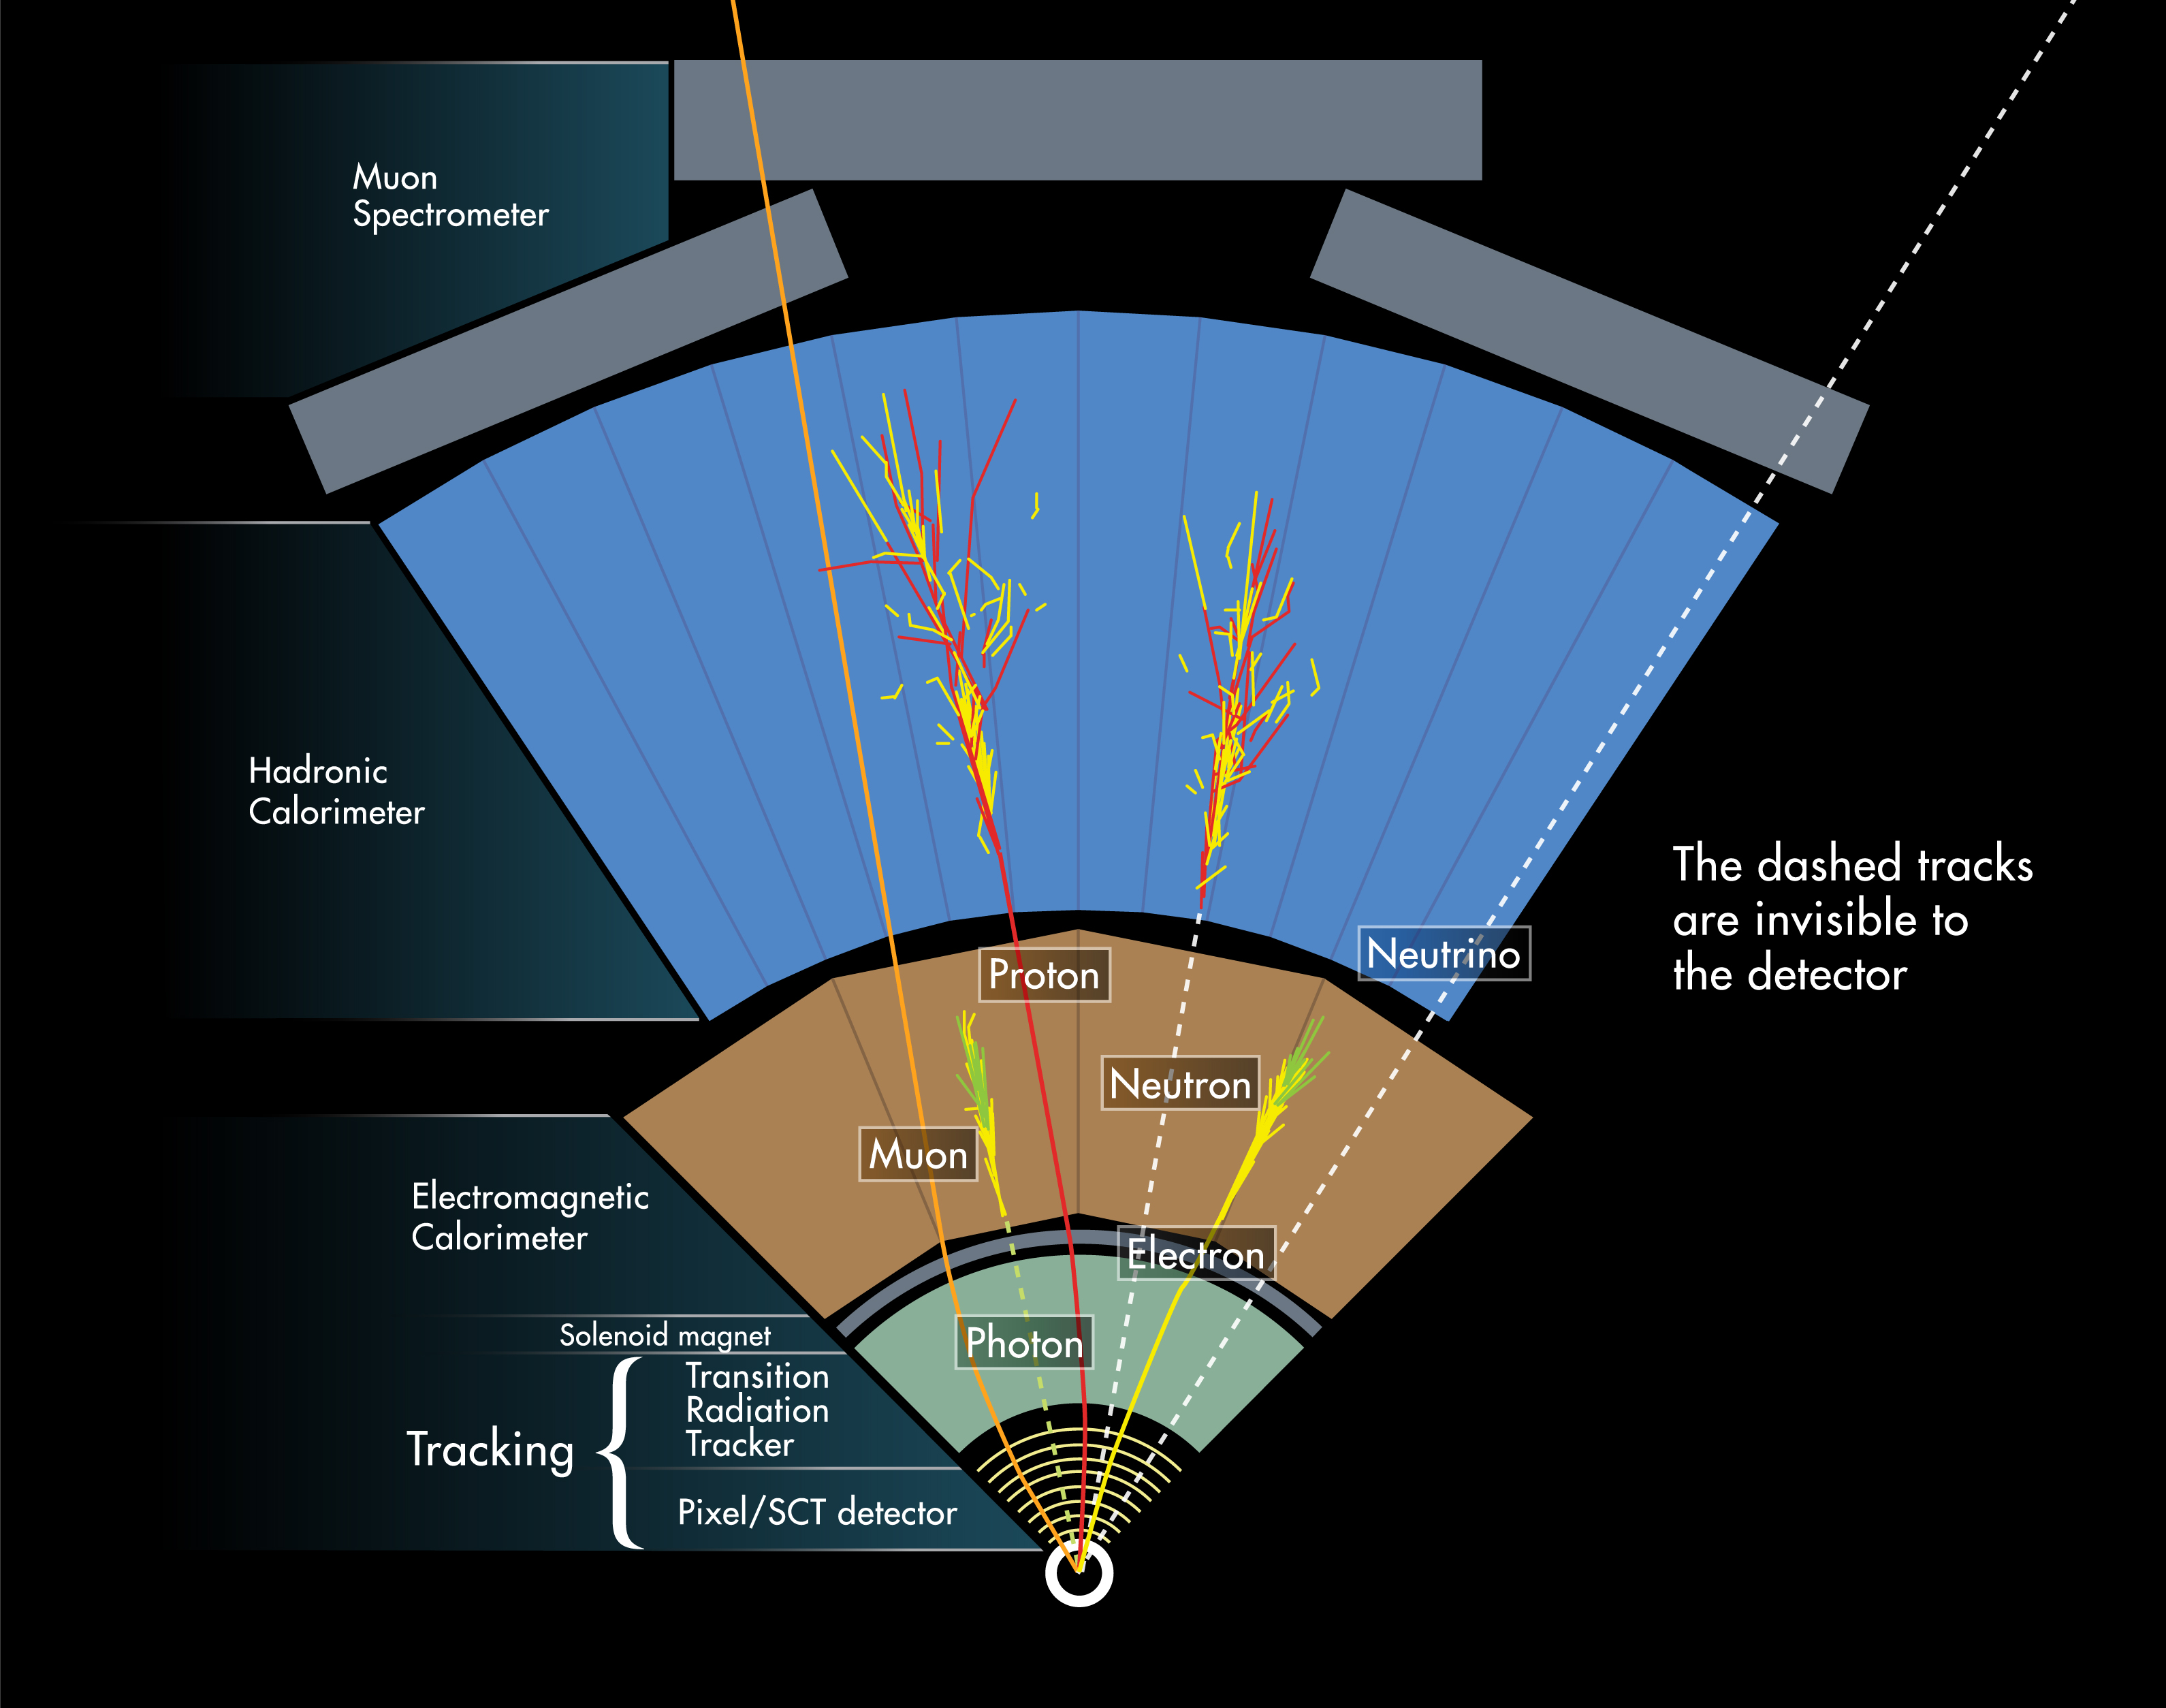
\includegraphics[width=0.6\textwidth]{figures/detector/ATLAS_particle}
   \caption{Illustration of particle interactions in ATLAS.}
  \label{fig:obj_reco_overview}
\end{figure}

%%%%%%%%%%%%%%
\section{ID Tracks and Vertices}
%\paragraph{}
%ID tracks originate from clusters based on PIXEL and SCT energy deposits.
%Three clusters form a seed, and the seeds are combined to build track candidates using a Kalman filter. 
%After ambiguity solving, an artificial neural network is used to identify merged clusters.
%Finally, ID tracks are built from CPU intensive high resolution fits.

\paragraph{}
Each beam crossing generates multiple vertices, and the vertices are reconstructed from the available ID tracks. 
The primary vertex (PV), or the hard-scatter vertex, is selected as the one with the largest $\sum p_T^2$, where the sum is over all tracks with transverse momentum $p_T > 0.4$ \GeV that are associated with the vertex.
The ID tracks are usually required to have at least 1 PIXEL hit and 6 SCT hits, and to be tightly matched to the primary vertex. 
The tracks are required to have $p_T > 0.4$ \GeV~ and $|\eta| < 2.5$.

\paragraph{}
The track reconstruction performance is highly dependent on the momentum of the particle. 
With higher momentum, the decay tracks have smaller separations in the inner detector, hindering the resolving cluster process, and thus degrading the track identification efficiency. 
For a $1$ \TeV~ $b$-hadron, the reconstruction track efficiency is $83\%$, compared to $95\%$ for a $200$ \GeV~ $b$-hadron ~\cite{Aaboud:2017all}.

%%%%%%%%%%%%%%
\section{Jets}
%% Jet talk: https://cds.cern.ch/record/2284807/files/ATL-PHYS-SLIDE-2017-781.pdf
\paragraph{}
When a quark or gluon is produced in $pp$ collisions, it produces a collimated spray of hadrons, which is known as a jet~\cite{Salam:2009jx}.
Jets are built from topological clusters of energy deposits in calorimeter cells \cite{PERF-2014-07}, using a four-momentum reconstruction scheme with massless clusters as input. 
The directions of jets are corrected to point back to the primary vertex.
Typically, jets are reconstructed using the \akt algorithm~\cite{AntiKt} with different values of the radius parameter \R.
\R appears in the denominator of the clustering distance metric. 
This favors clusterings that involve hard particles, and the jets grow outwards around hard ``seeds''.
It determines the radial size of the jet in $\eta$-$\phi$ plane.

\subsection{Small-\R jets}
\paragraph{}
The jets with $R=0.4$ (``small-\R jets'') are reconstructed from clusters calibrated at the electromagnetic (EM) scale. The jets are corrected for additional energy deposited from pile-up interactions using an area-based correction \cite{Cacciari:2008gn}. 
They are then calibrated using \pt- and $\eta$-dependent calibration factors derived from simulation, before global sequential calibration~\cite{Aad:2011he} is applied, which reduces differences in calorimeter responses to gluon or quark-initiated jets. 
The final calibration is based on in situ measurements in collision data~\cite{ATL-PHYS-PUB-2015-015}.

\paragraph{}
``Small-\R jets'' are required to be consistent with the primary vertex, in order to avoid contamination from pileup interactions. 
The jet vertex fraction (JVF) is a useful variable for this purpose. 
It is the ratio of tracks associated with a primary vertex to the total number of tracks inside a jet. 
Jets from the PV should have most tracks consistent with the PV and therefore have a large JVF value.
 %Jets with $p_T<60$~\GeV\, $|\eta|<2.4$, and with a large fraction of their energy arising from pile-up interactions are suppressed using tracking information, which was combined in a multivariate classification algorithm (\emph{jet vertex tagger})~\cite{ATL-PHYS-PUB-2014-001}. 
 %Events that pass a ``medium'' jet vertex tagger working point, corresponding to a 92\% efficiency for jets at the EM scale with $20<p_T<60$~\GeV, are retained in the analysis. 
 %Quality criteria are applied to the jets, and events with jets consistent with noise in the calorimeter or non-collision backgrounds are vetoed~\cite{jetcleanATLAS}.

\subsection{Large-\R jets}
\label{obj:largeRjet}
%% If add plots, use 
%% https://atlas.web.cern.ch/Atlas/GROUPS/PHYSICS/CONFNOTES/ATLAS-CONF-2017-063/
%% Nice talk: https://cds.cern.ch/record/2275665/files/ATL-PHYS-SLIDE-2017-577.pdf

\begin{figure}[htbp!]
  \centering
  \captionsetup{justification=centering}
  \hspace{-3cm}
    \begin{subfigure}[b]{0.35\textwidth}
        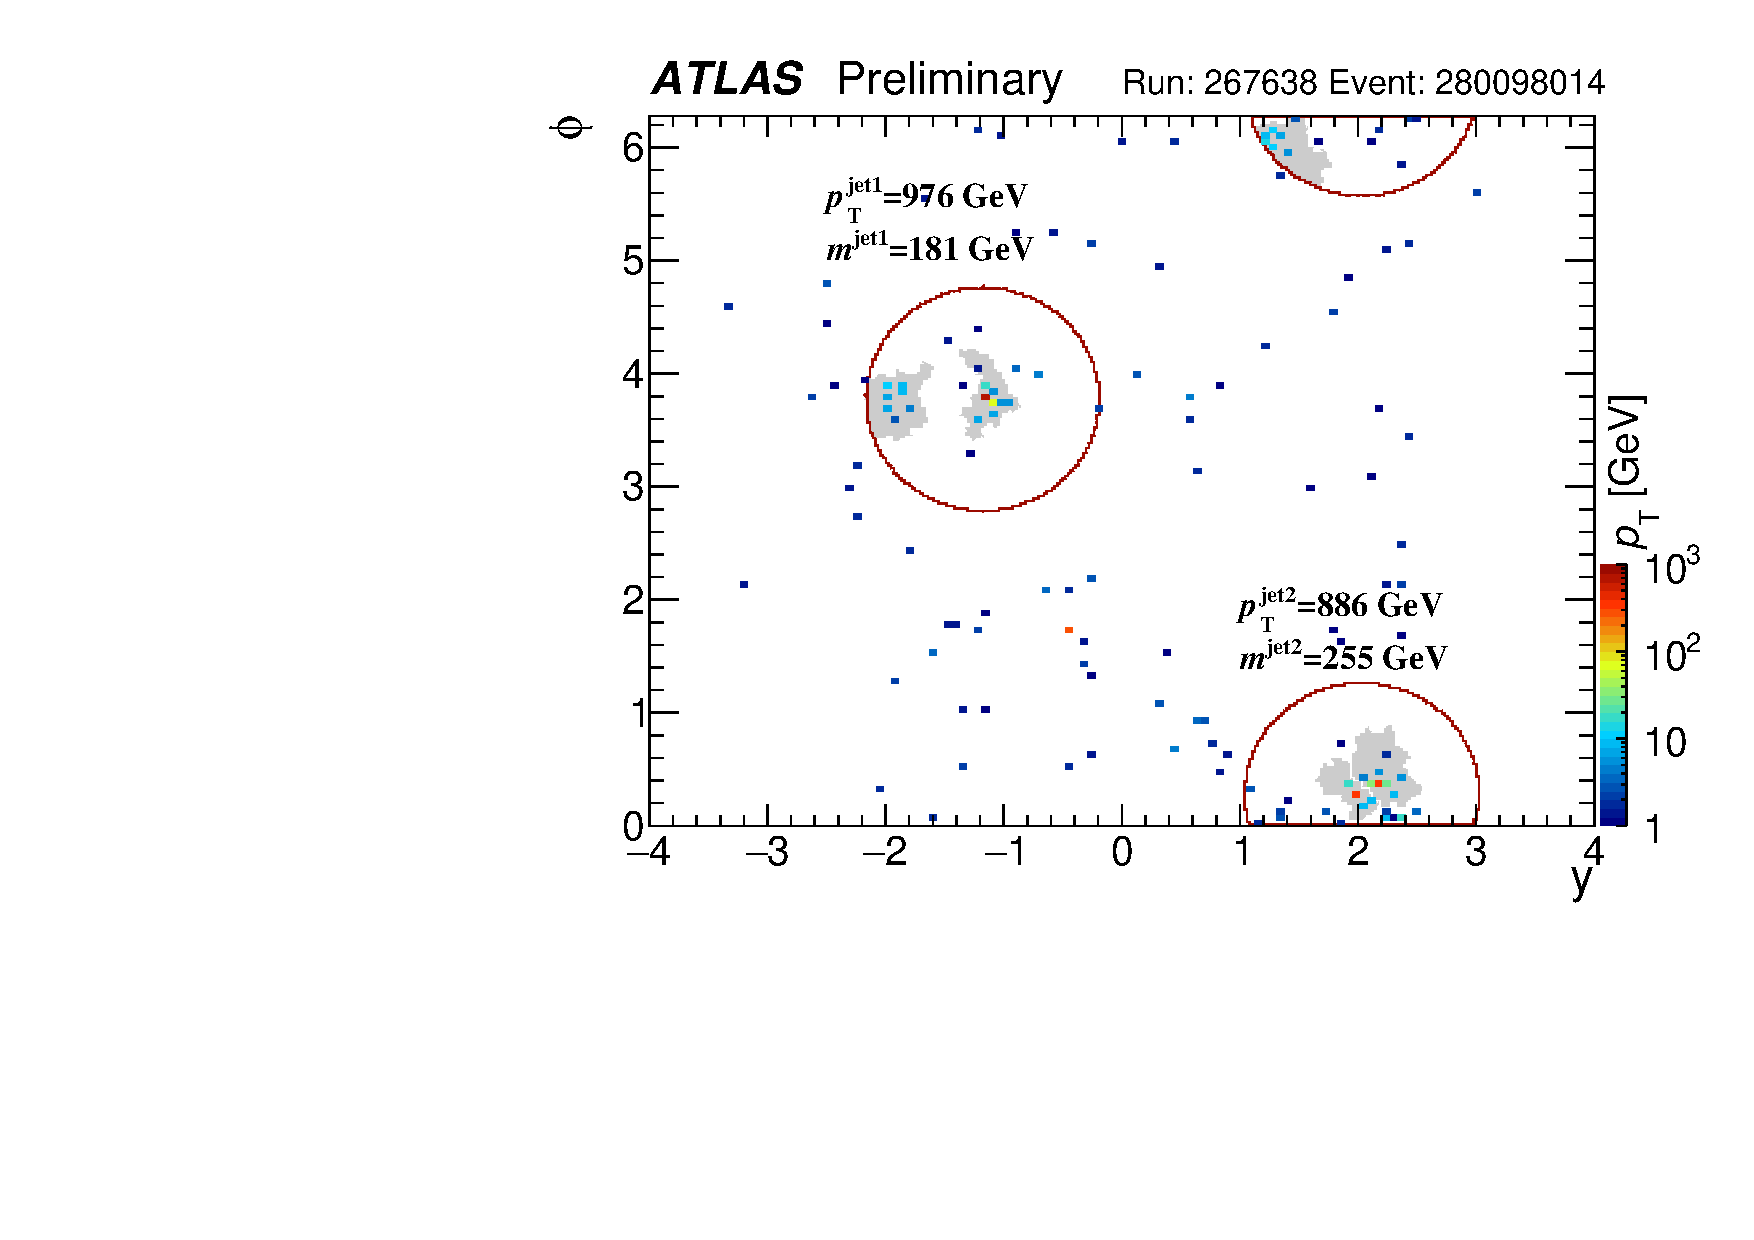
\includegraphics[width=\textwidth,angle=-90]{figures/object/Jet_evt_a.pdf}
        \caption{Event 28009014}
        \label{fig:obj_jet_evt_a}
    \end{subfigure}
    \quad \quad \quad \quad
    \begin{subfigure}[b]{0.35\textwidth}
        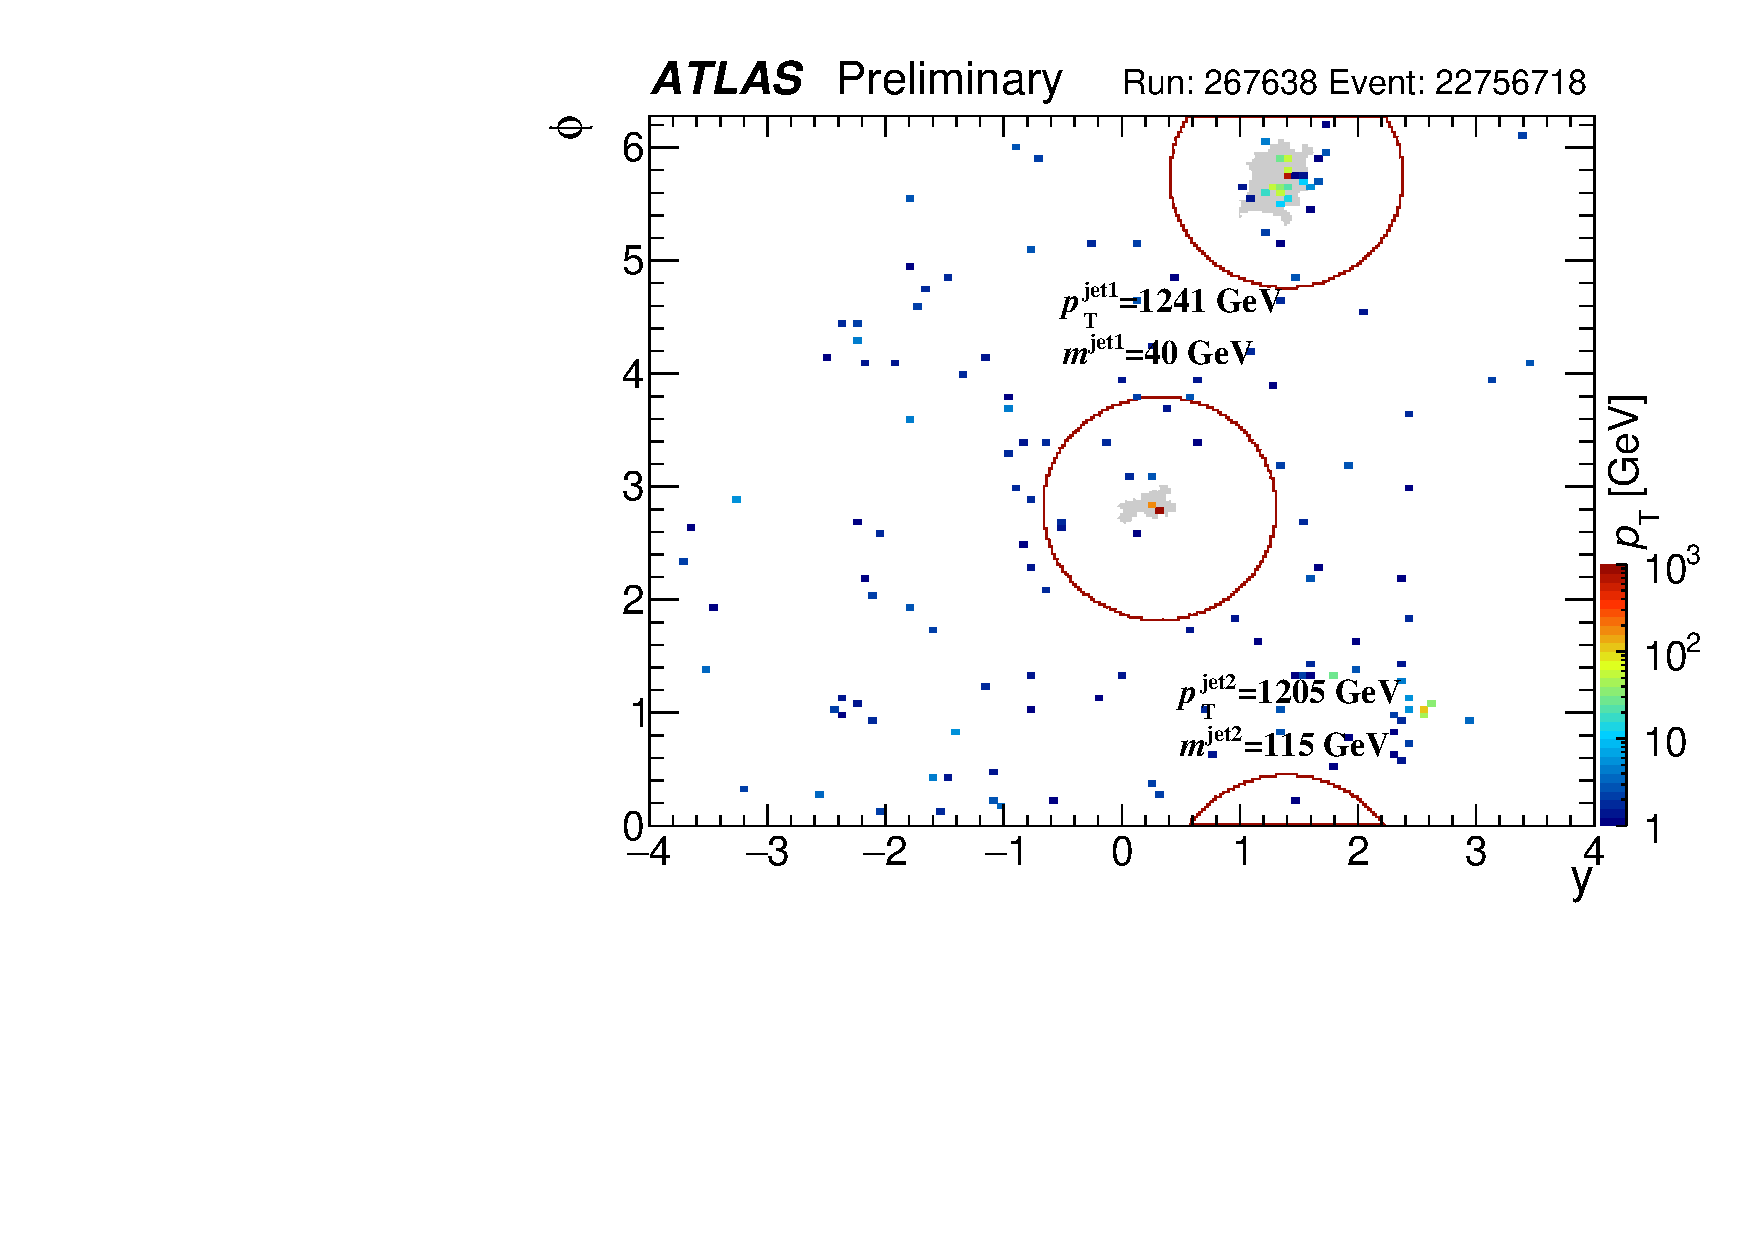
\includegraphics[width=\textwidth,angle=-90]{figures/object/Jet_evt_b.pdf}
        \caption{Event 22756718}
        \label{fig:obj_jet_evt_b}
    \end{subfigure}
   \caption{
   Two collision events recorded in June 2015 with a high leading jet \pt shown in rapidity-azimuthal angle parameter space. 
   The dots are calorimeter-cell clusters with positive energy. 
   Only the two leading jets are shown, with their area demarcated by a colored circle, and with grey regions denoting the corresponding \kt~ sub-jets of size $R_{sub}=0.2$. 
   The colour of both jets and clusters corresponds to their \pt.}
  \label{fig:obj_jet_evt}
\end{figure}

\paragraph{}
The jets with $R=1.0$ (``large-\R jets'') are built from locally calibrated~\cite{Aad:2011he} topological clusters.
Two examples are shown in Figure~\ref{fig:obj_jet_evt}~\cite{ATLAS-CONF-2015-035}.
Large-\R jets are trimmed~\cite{Krohn2010} to minimize the impact of contamination from non-perturbative effects associated with beam-remnants (``pile-up'' events).
Trimming proceeds by reclustering the jet with the \kt~ algorithm~\cite{Ellis:1993tq} into $R_{sub} = 0.2$ sub-jets and then removing those sub-jets with $p_T^{\mathrm{subjet}}/p_T^{\mathrm{jet}} < 0.05$, where $p_T^{\mathrm{subjet}}$ is the transverse momentum of the sub-jet and $p_T^{\mathrm{jet}}$ that of the original jet.
Trimming increases the jet mass resolution, as shown in Figure~\ref{fig:obj_trim}~\cite{ATL-PHYS-PUB-2017-020}.
The energy and mass scales of the trimmed jets are then calibrated using \pt- and $\eta$-dependent calibration factors derived from simulation~\cite{PERF-2012-02}.

\begin{figure}[htbp!]
  \centering
  \captionsetup{justification=centering}
    \begin{subfigure}[b]{0.4\textwidth}
        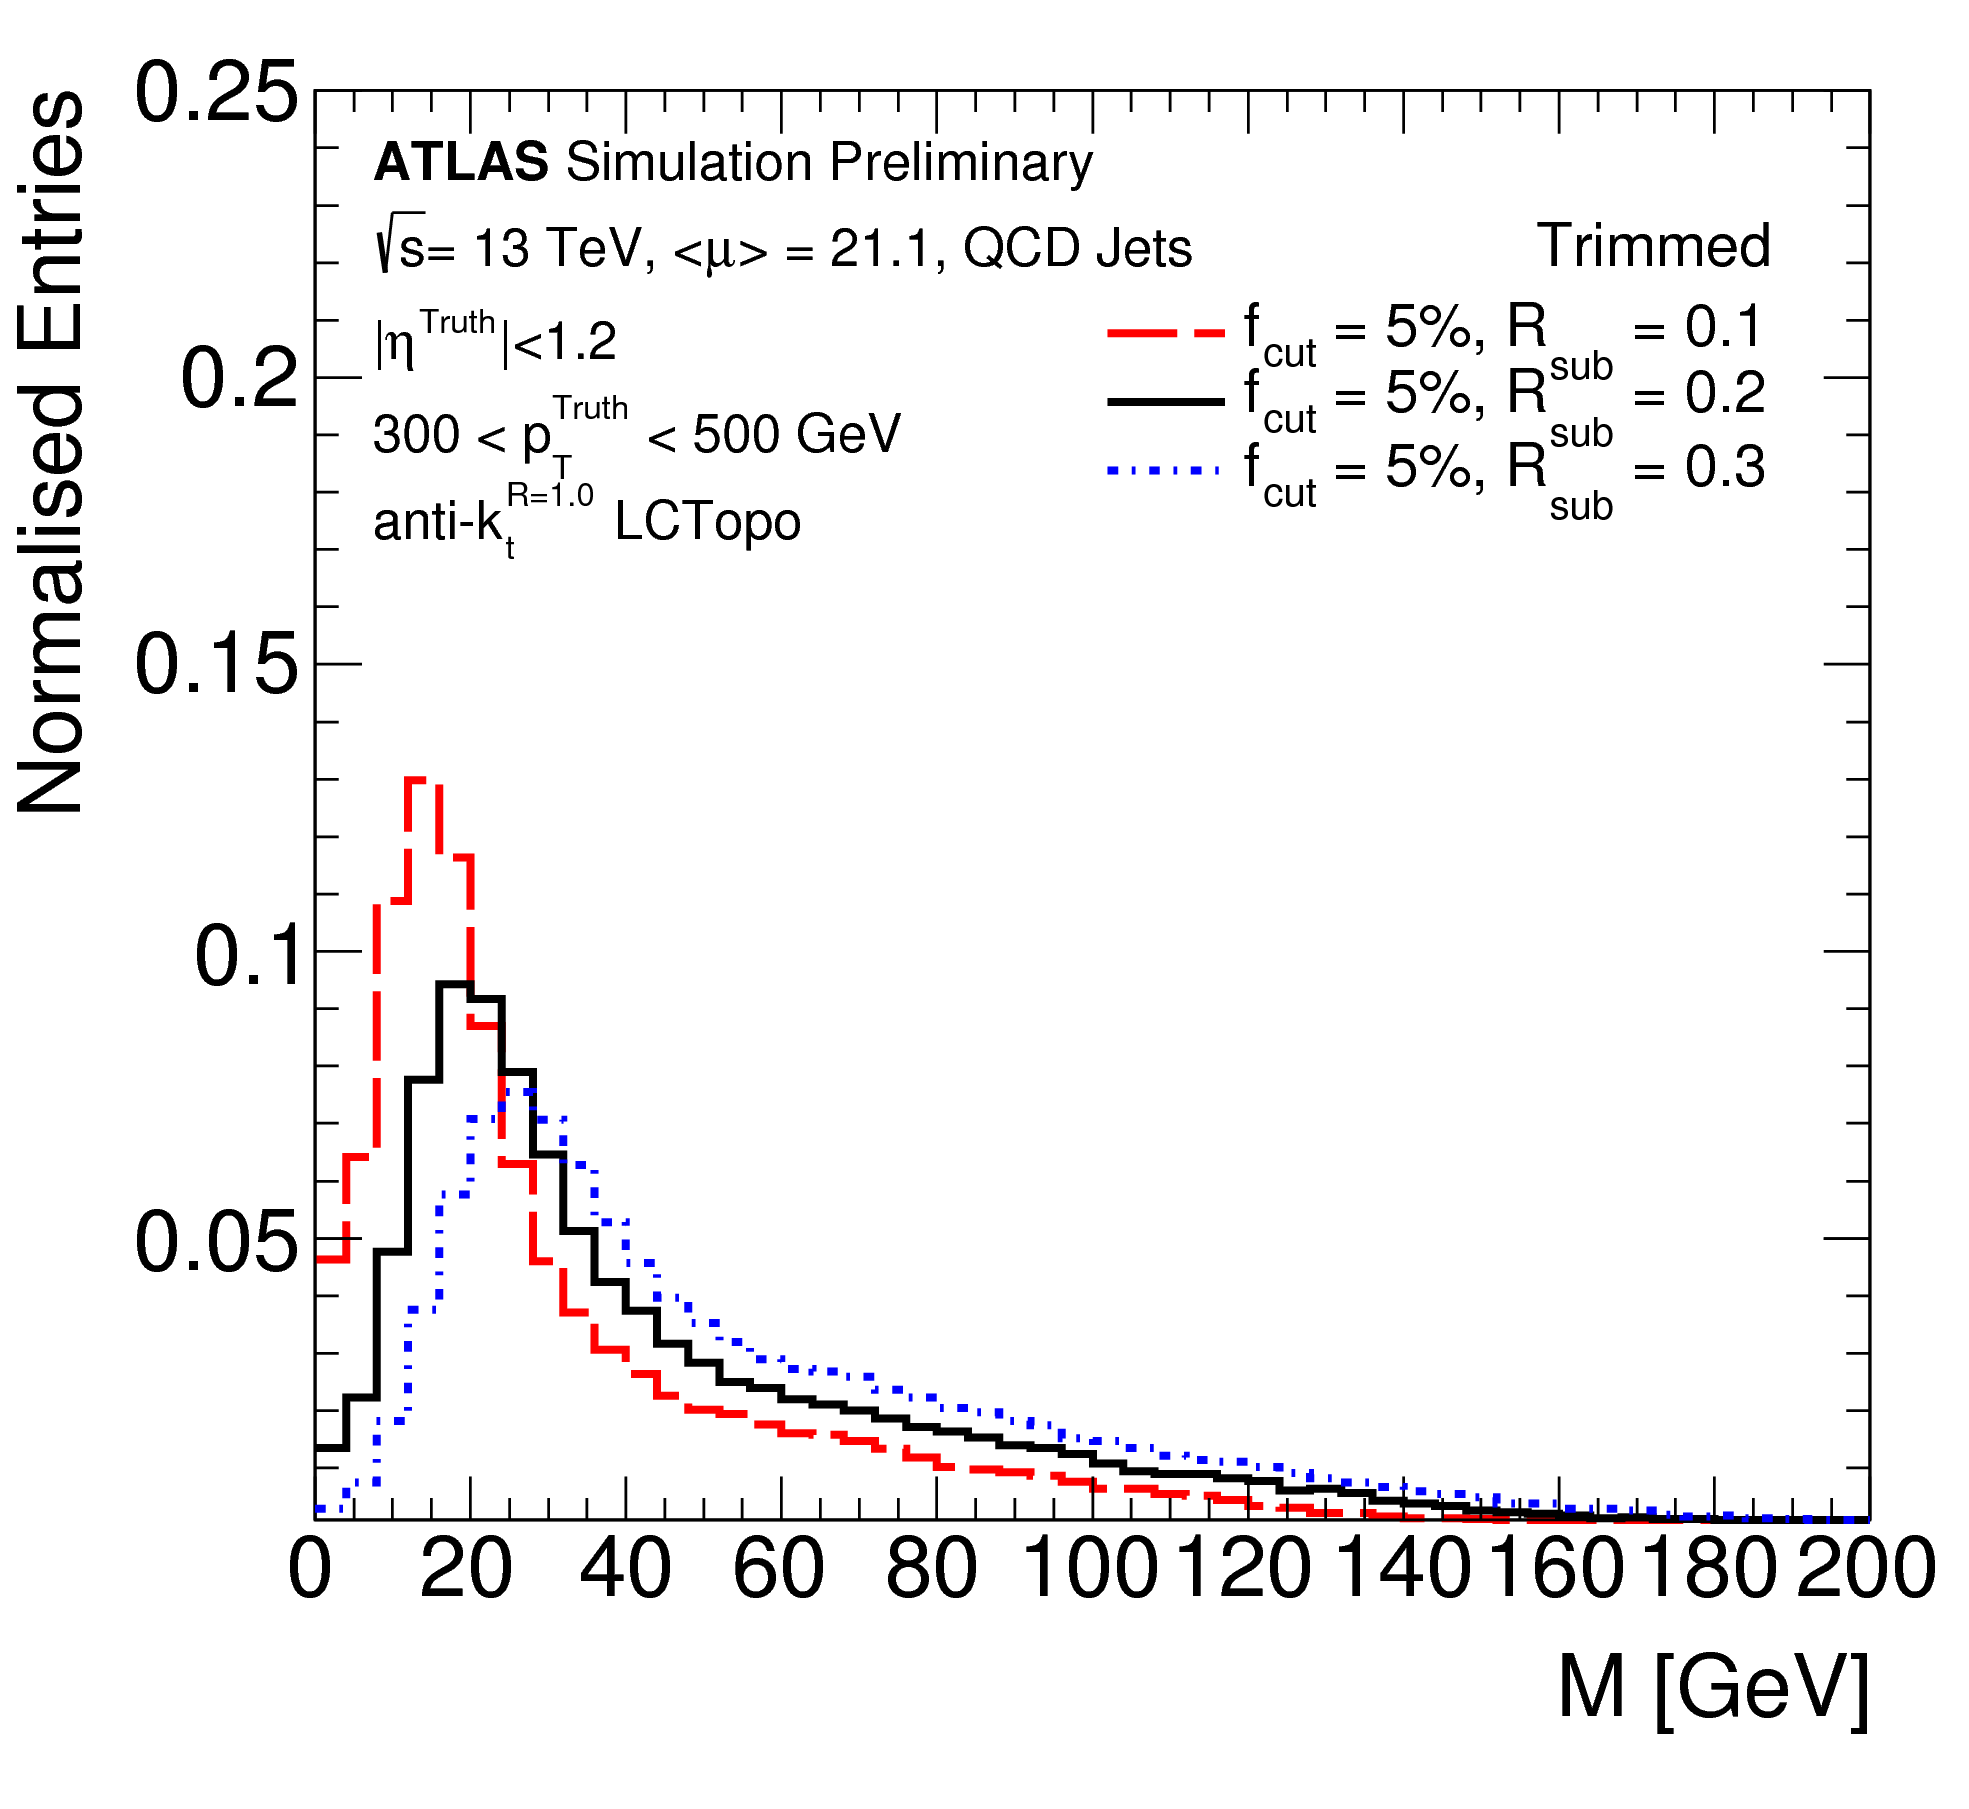
\includegraphics[width=\textwidth]{figures/object/trim_qcd_lowpt}
        \caption{QCD jets, $300 < p_{T} < 500$ \GeV}
        \label{fig:obj_trim_qcd_lowpt}
    \end{subfigure}
    \quad \quad 
    \begin{subfigure}[b]{0.4\textwidth}
        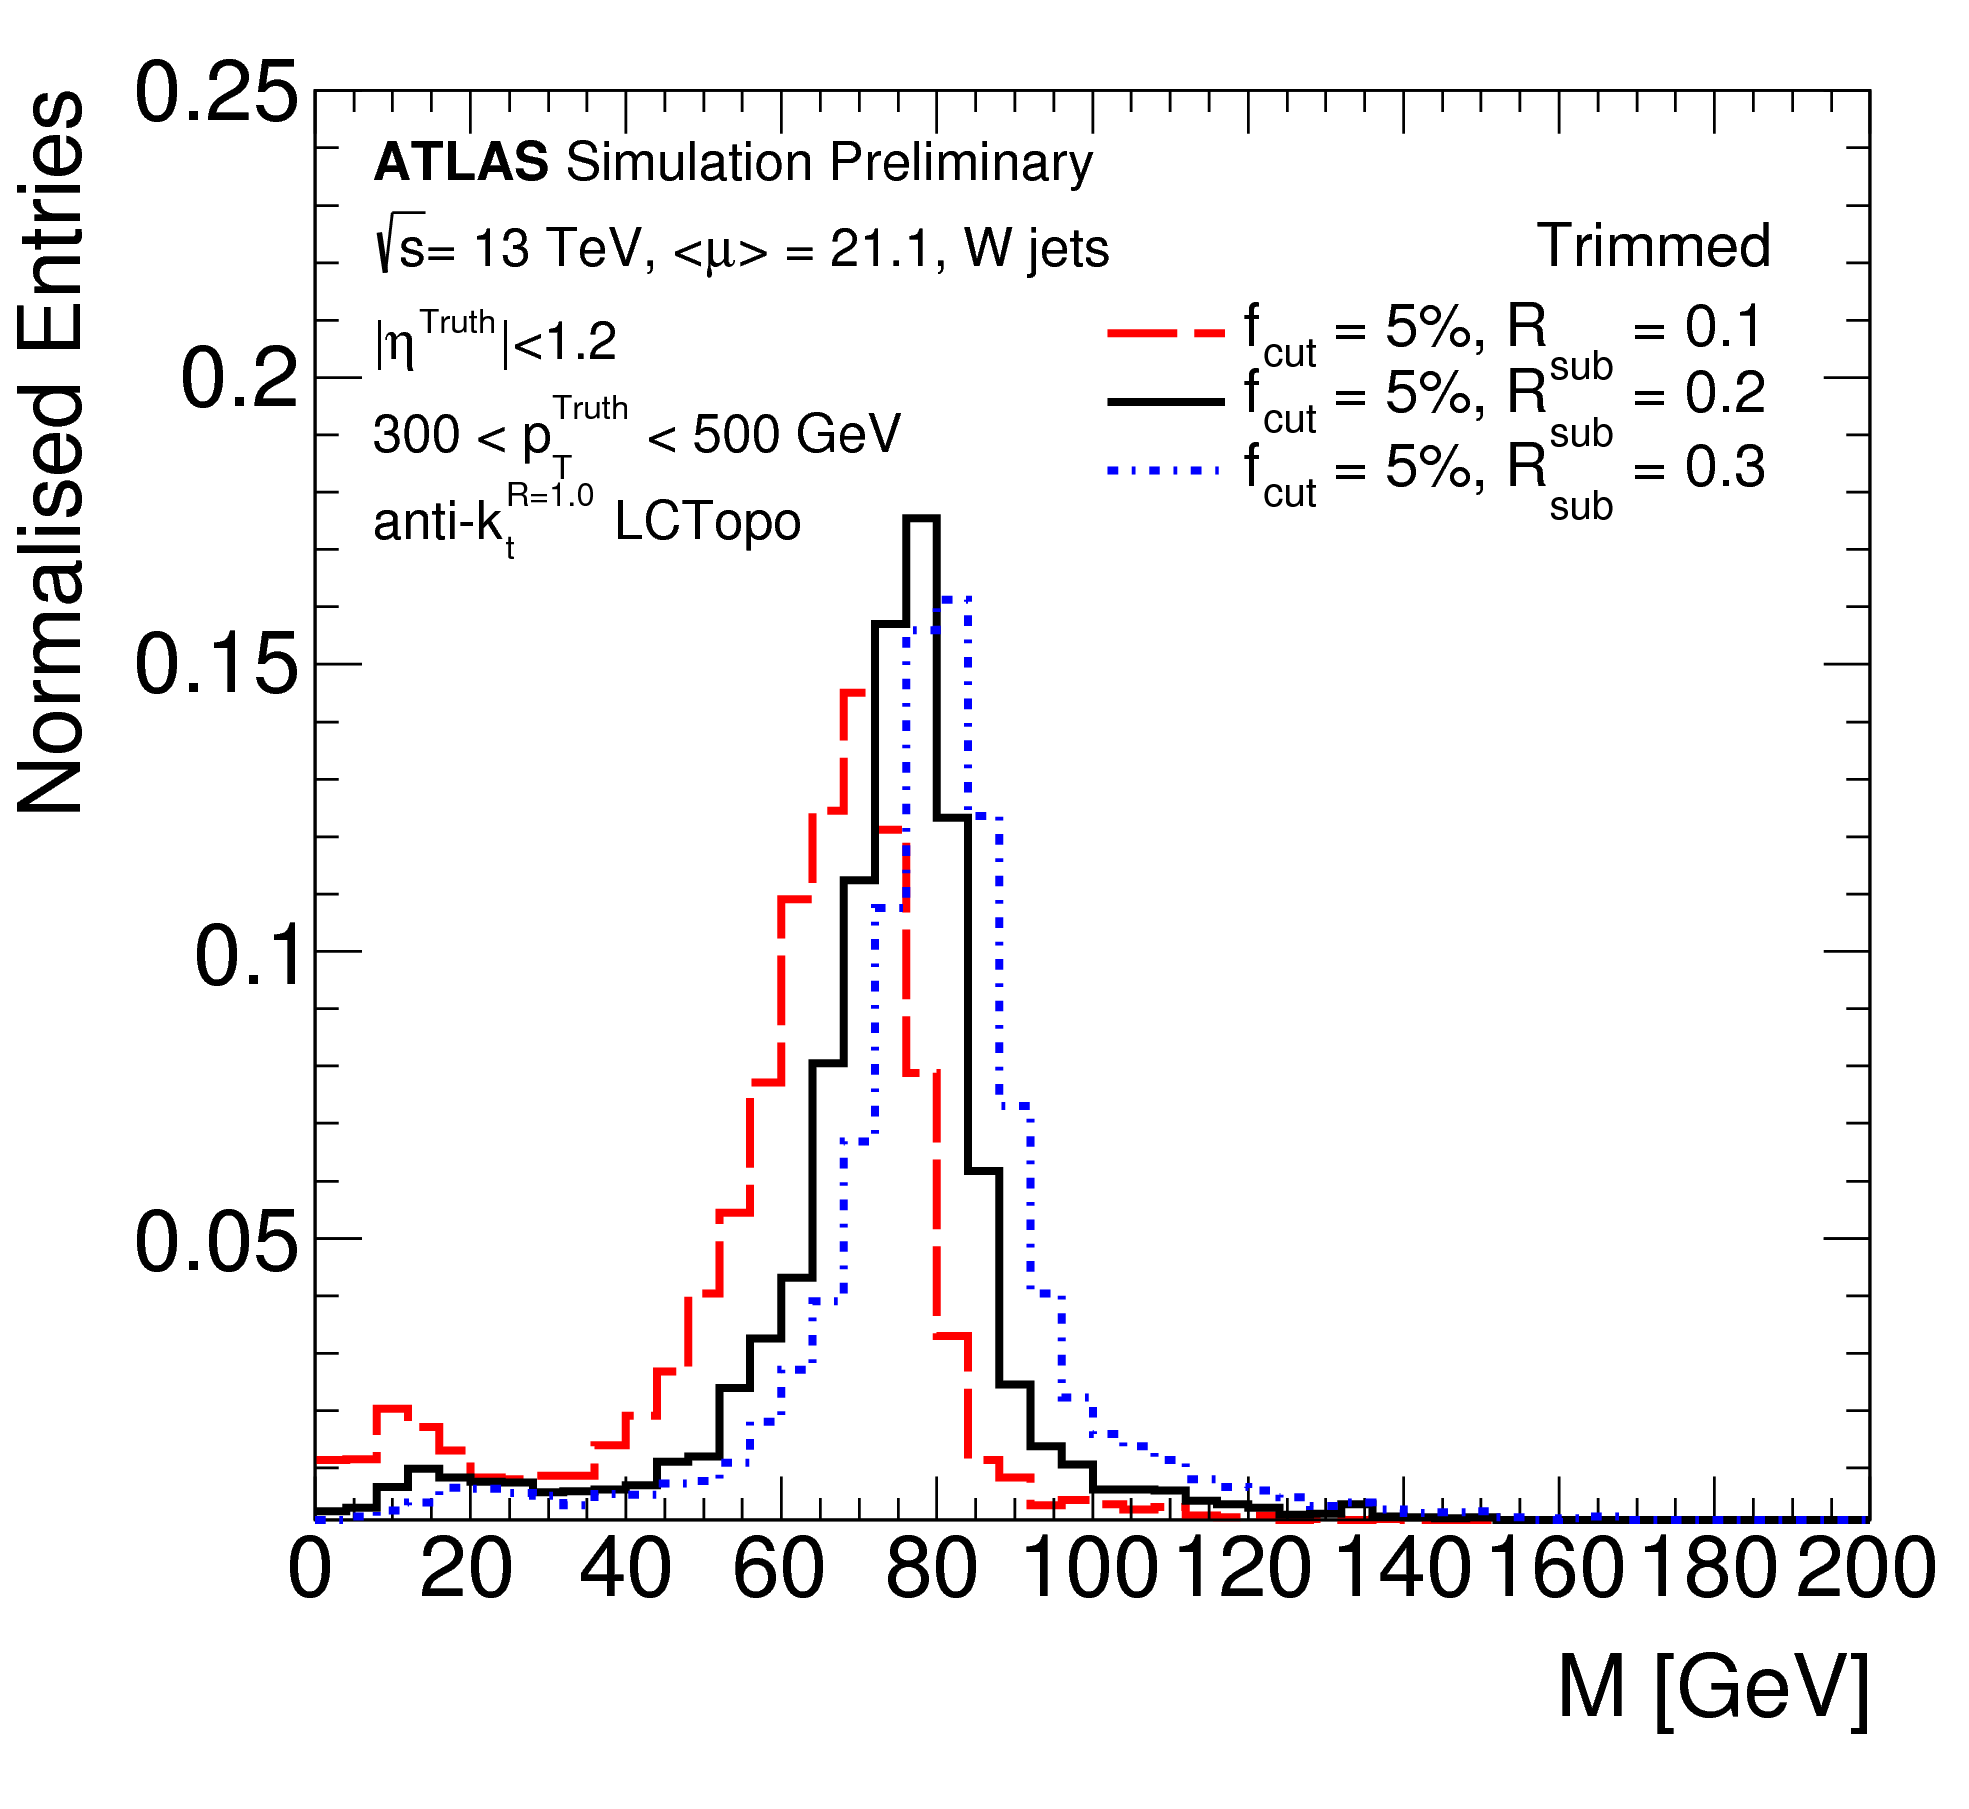
\includegraphics[width=\textwidth]{figures/object/trim_w_lowpt}
        \caption{$W$ jets, $300 < p_{T} < 500$ \GeV}
        \label{fig:obj_trim_w_lowpt}
    \end{subfigure} \\ 
    \begin{subfigure}[b]{0.4\textwidth}
        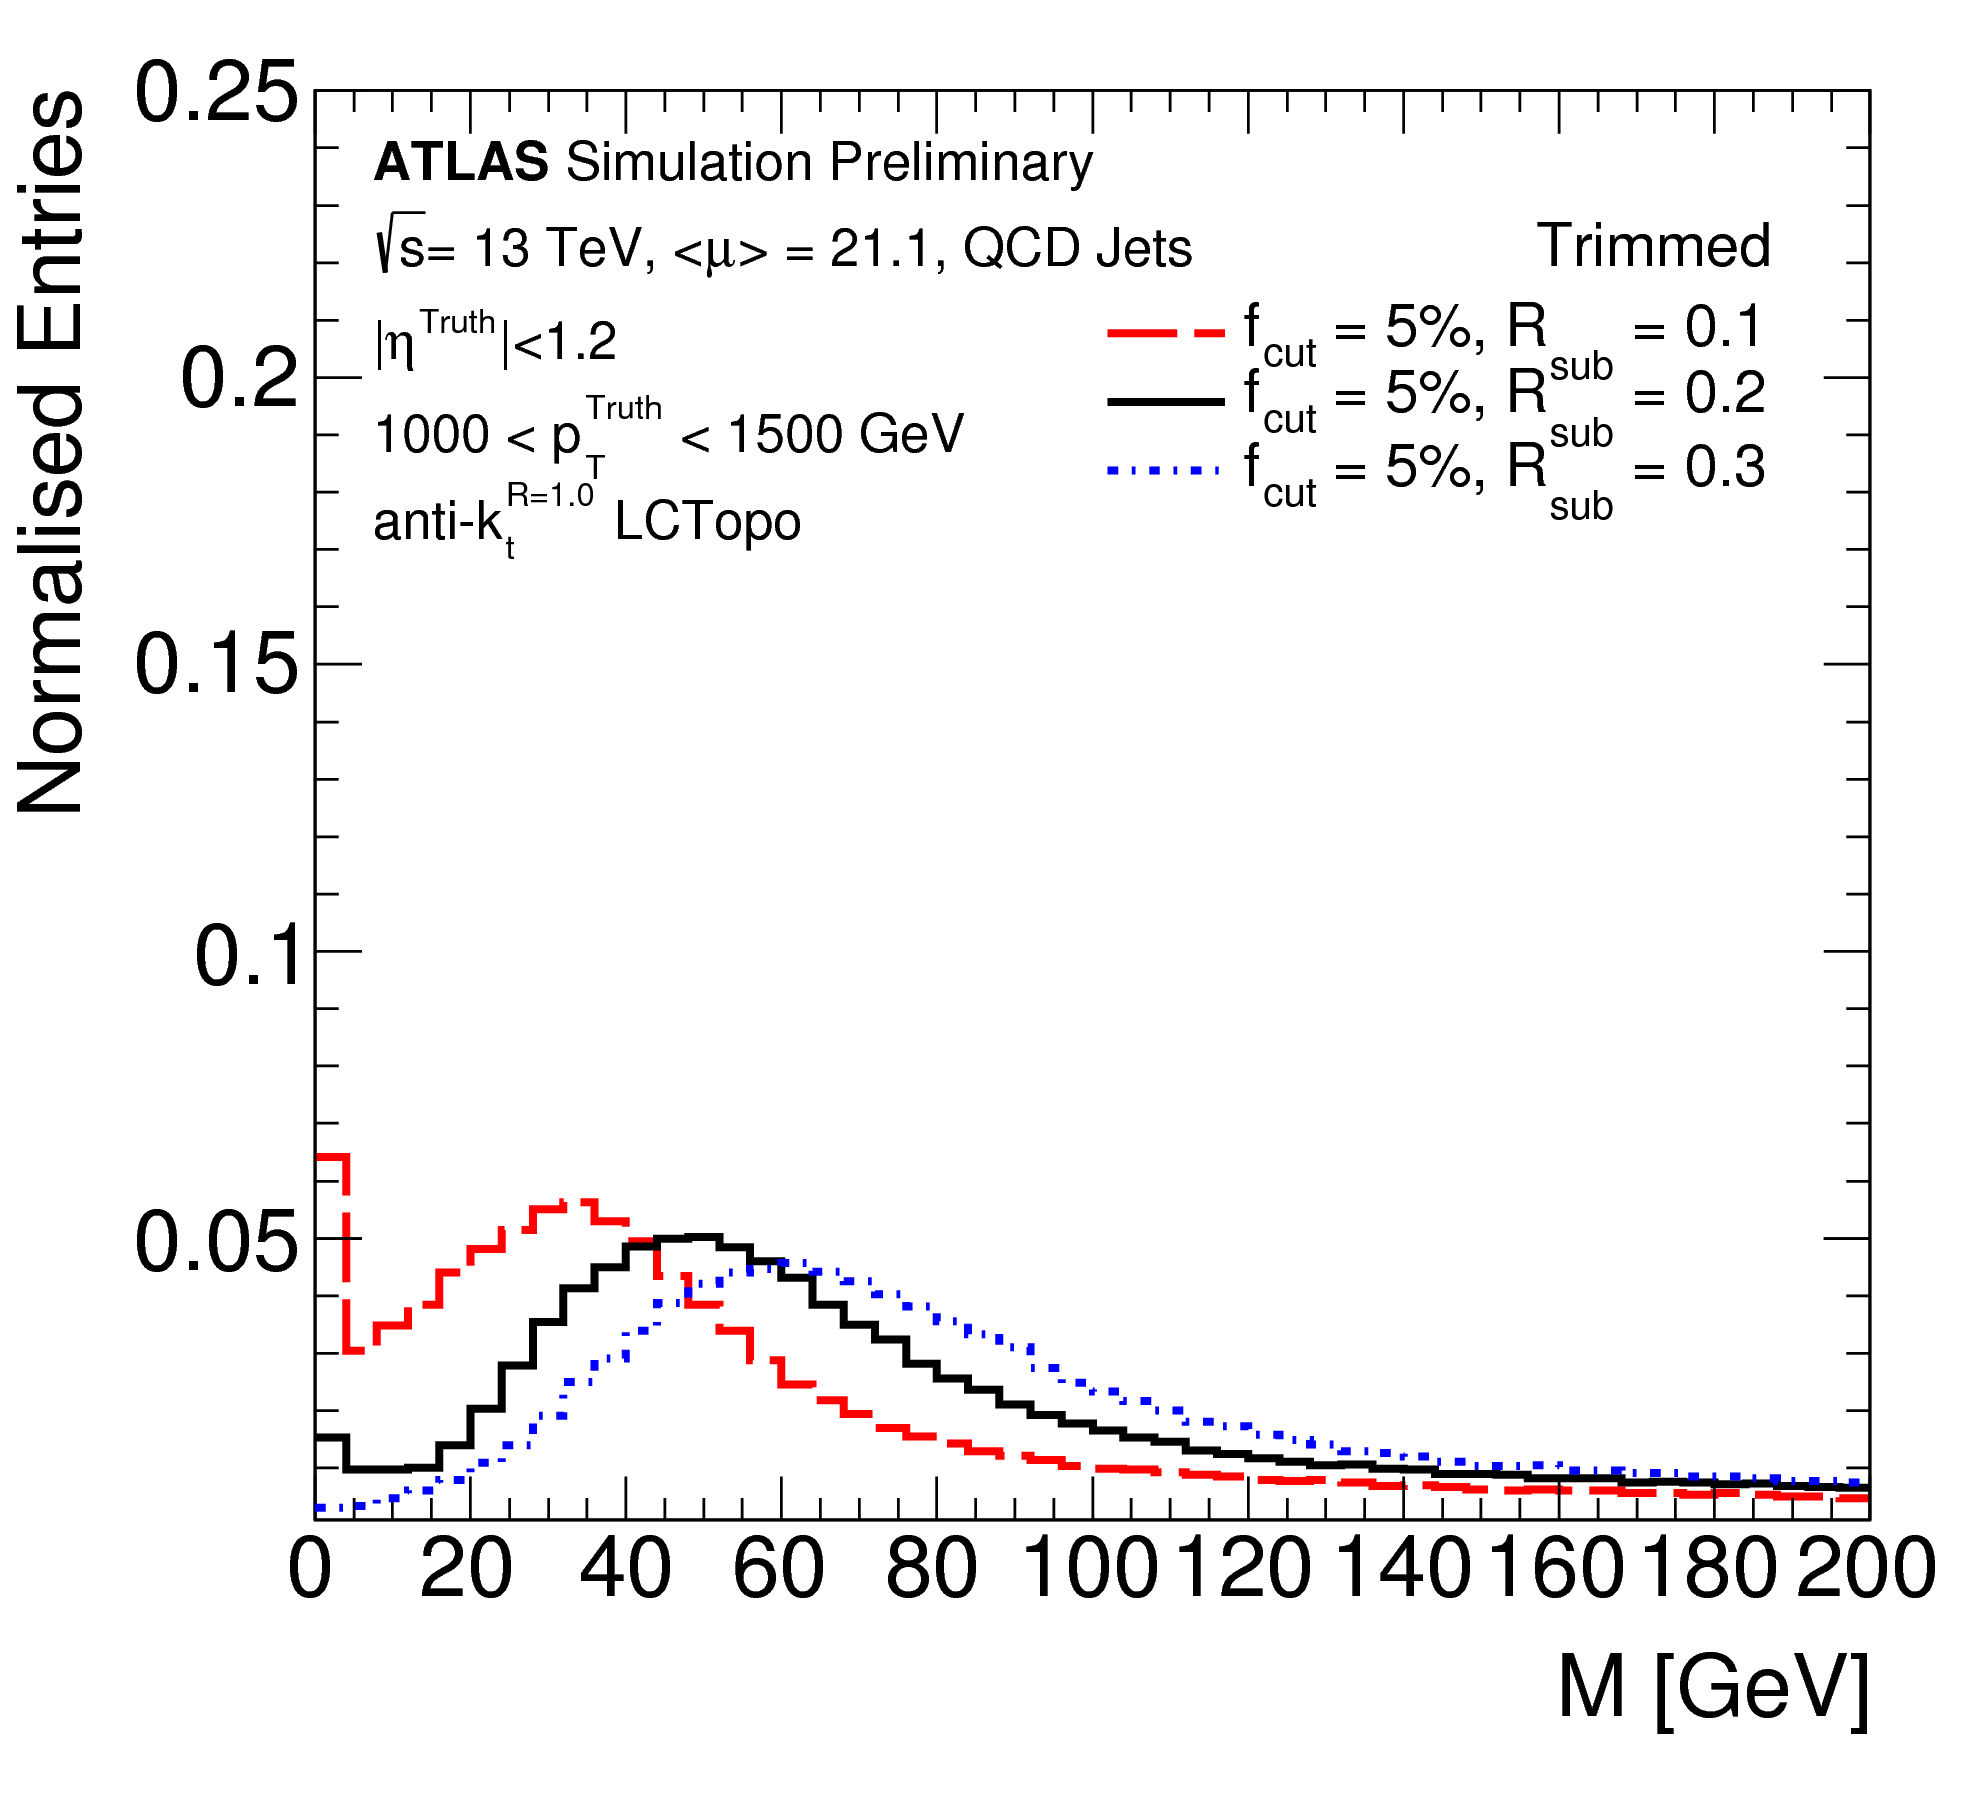
\includegraphics[width=\textwidth]{figures/object/trim_qcd_highpt}
        \caption{QCD jets, $1000 < p_{T} < 1500$ \GeV}
        \label{fig:obj_trim_qcd_highpt}
    \end{subfigure}
    \quad \quad 
    \begin{subfigure}[b]{0.4\textwidth}
        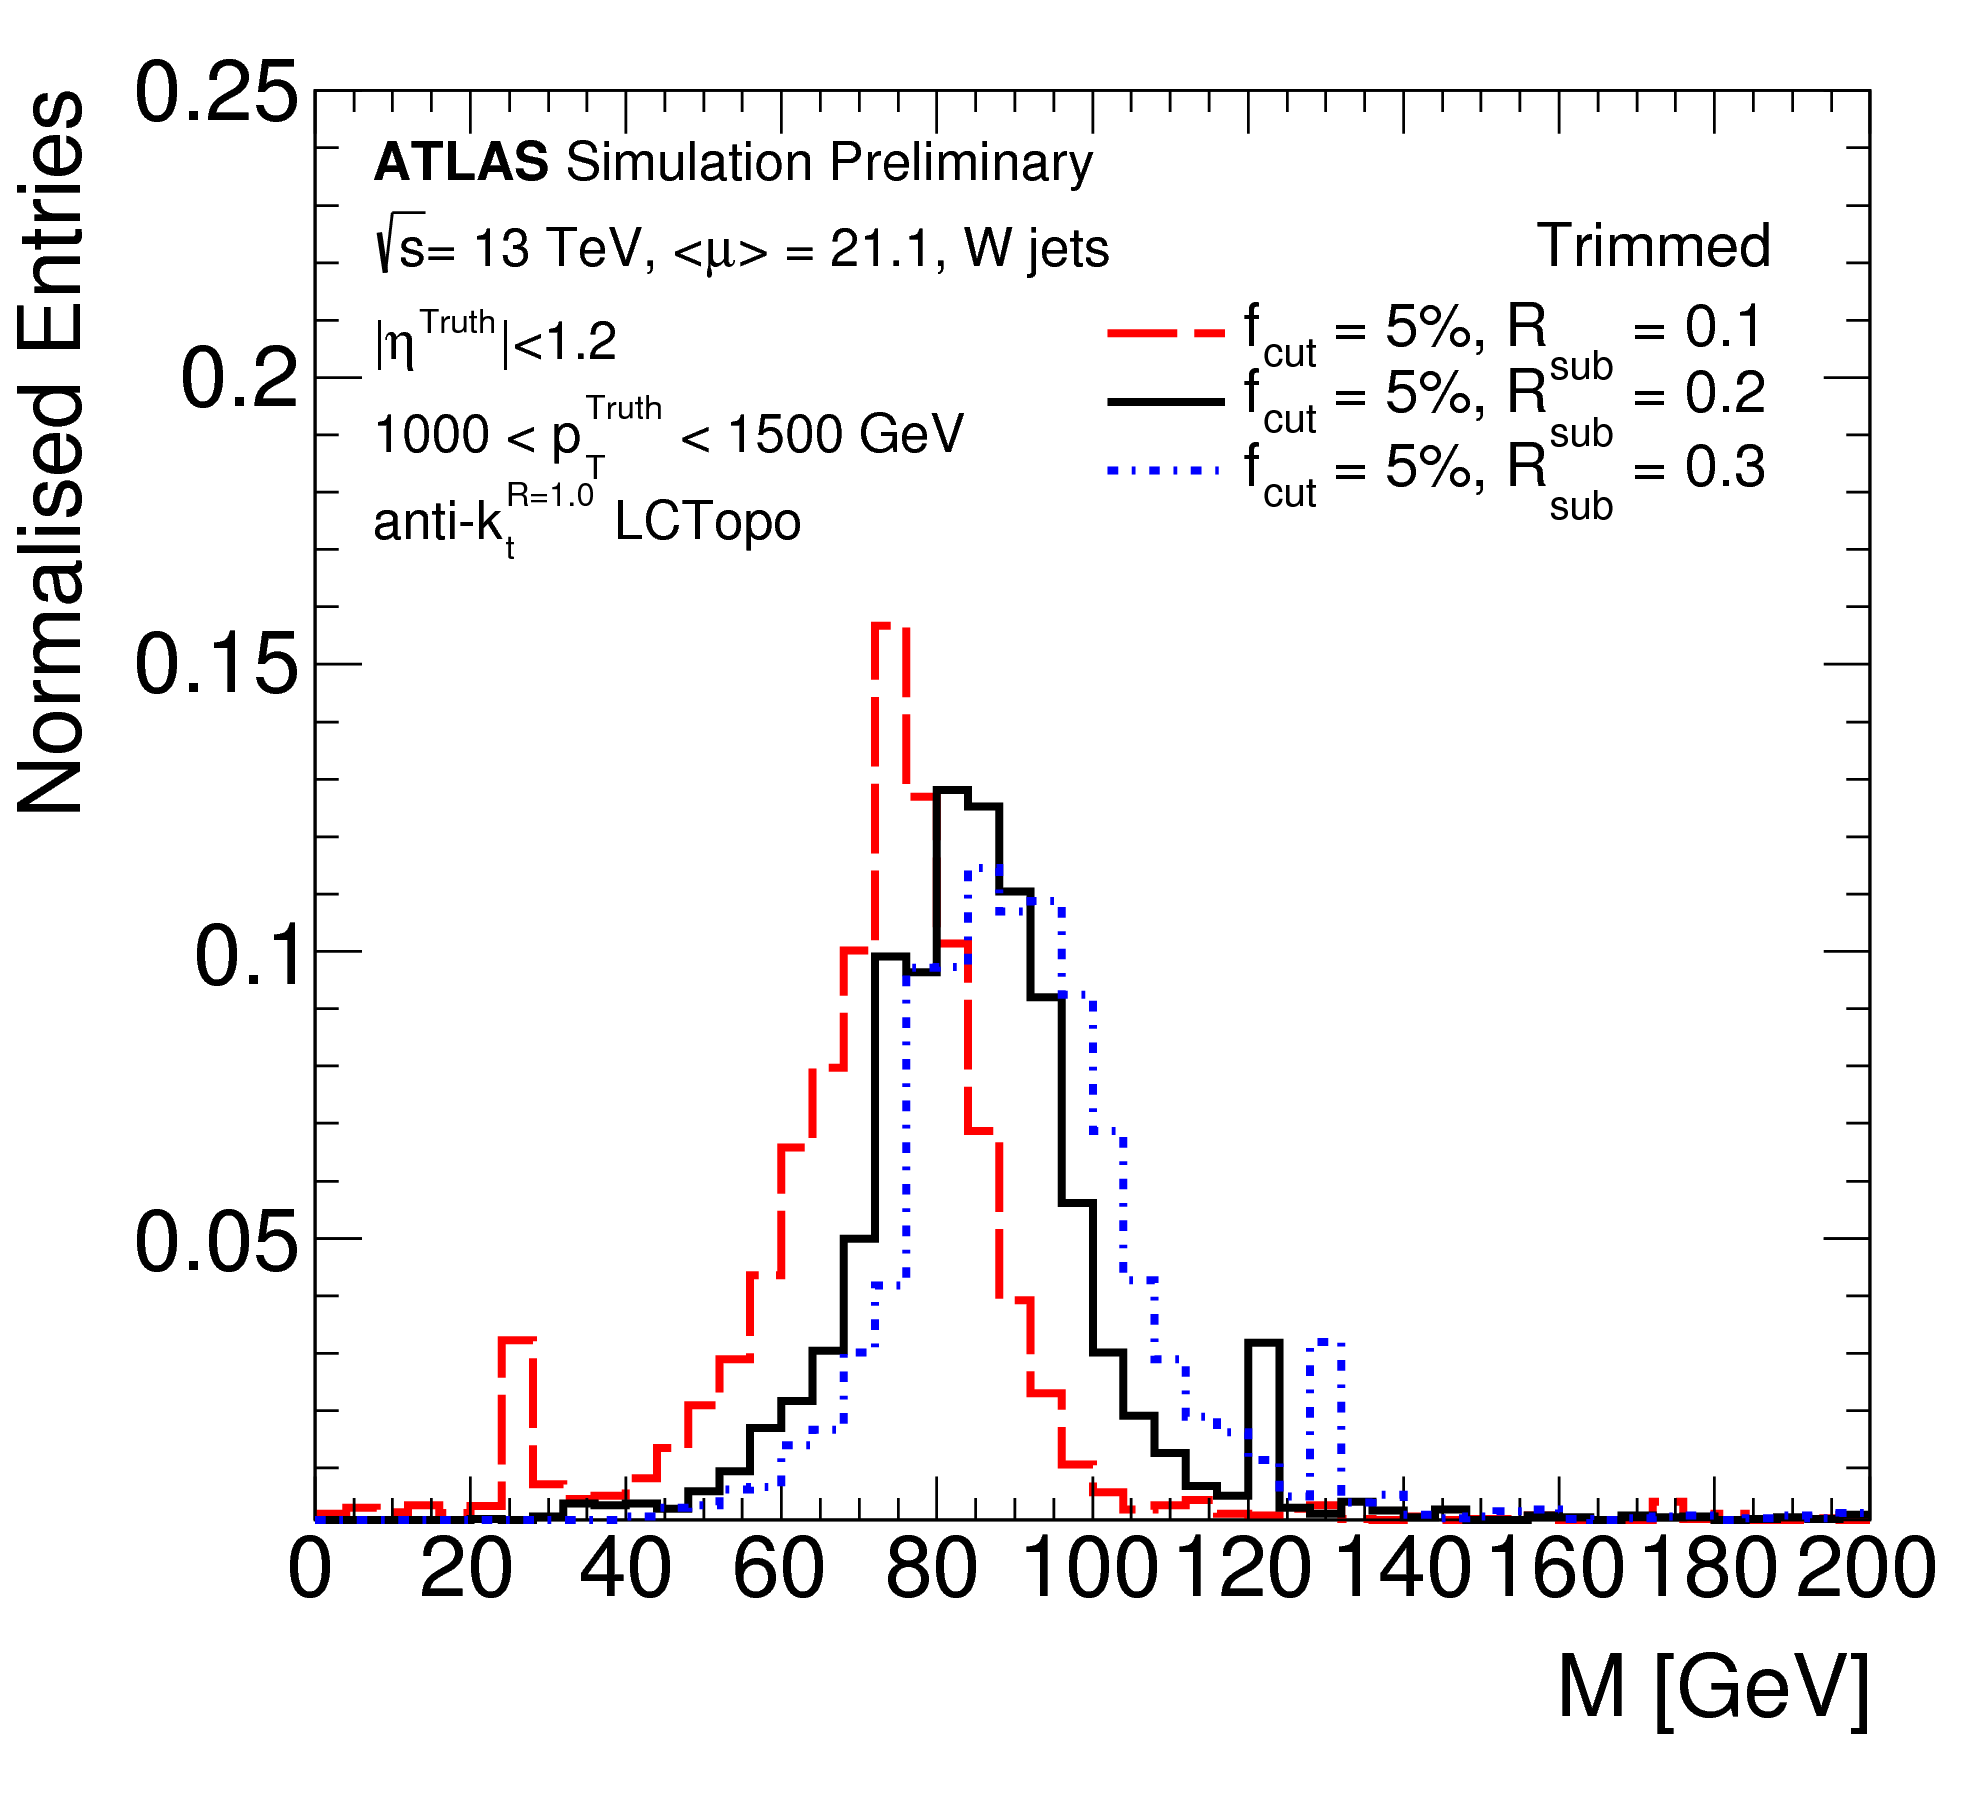
\includegraphics[width=\textwidth]{figures/object/trim_w_highpt}
        \caption{$W$ jets, $1000 < p_{T} < 1500$ \GeV}
        \label{fig:obj_trim_w_highpt}
    \end{subfigure} \\ 
   \caption{
   For the trimming algorithm using calorimeter cell clusters as inputs to the \akt jet reconstruction algorithm with $R = 1.0$, a comparison of the jet mass distribution for QCD background jets and $W$ boson jets low \pt~ and high \pt~ kinematic regions, as determined by the untrimmed truth jet \pt~. 
   The trimming parameter choices shown here are $R_{sub} = 0.1$, $0.2$, and $0.3$ for a fixed cut at $5\%$.}
  \label{fig:obj_trim}
\end{figure}

%Melissa asked me this question on Feb 13, 2017.
\paragraph{}
The calorimeter-based jet mass $m^{calo}$ for  a large-radius calorimeter jet $J$ is computed from the calorimeter cell cluster constituents $i$ with energy $E_i$ and momentum $p_i$:
\begin{equation}
m^{calo} = \sqrt{\left(\sum_{i\in J}E_i\right)^2-\left(\sum_{i\in J}\vec{p}_i\right)^2}.
\end{equation}

\paragraph{}
%For a $b$ quark, the angular spread in the decay products scales as $\frac{1}{p_T}$. 
%It is comparable with the $\eta\times\phi \sim 0.1\times0.1$ calorimeter granularity for a highly boosted $b$.
Tracking information is used to increase the mass resolution.
The track-assisted jet mass, $m^{TA}$, is defined as:
\begin{equation}
m^{TA} = \frac{p_T^{calo}}{p_T^{track}} \cdot m^{track}.
\end{equation}
where $p_{T}^{calo}$ is the transverse momentum of the large-\R calorimeter jet, $p_{T}^{track}$ is the transverse momentum of the four-vector sum of tracks associated to the large-\R calorimeter jet, and $m^{track}$ is the invariant mass of this four-vector sum.
This ratio corrects for charged-to-neutral hadron fluctuations, and therefore improves the resolution with respect to track-only jet mass.
%Ghost association is performed to associate tracks to the jets before the trimming procedure is applied.
%The fractional resolution is defined 0.5 \times 68 \% IQnR(Rm)∕median(Rm), where 68 \% IQnR(Rm) is the 68 \% confidence interval interquartile range of the jet mass response distribution, and median(Rm) is the median jet mass response.

\begin{figure}[htbp!]
  \centering
  \captionsetup{justification=centering}
	\hspace{-2cm}
    \begin{subfigure}[b]{0.45\textwidth}
        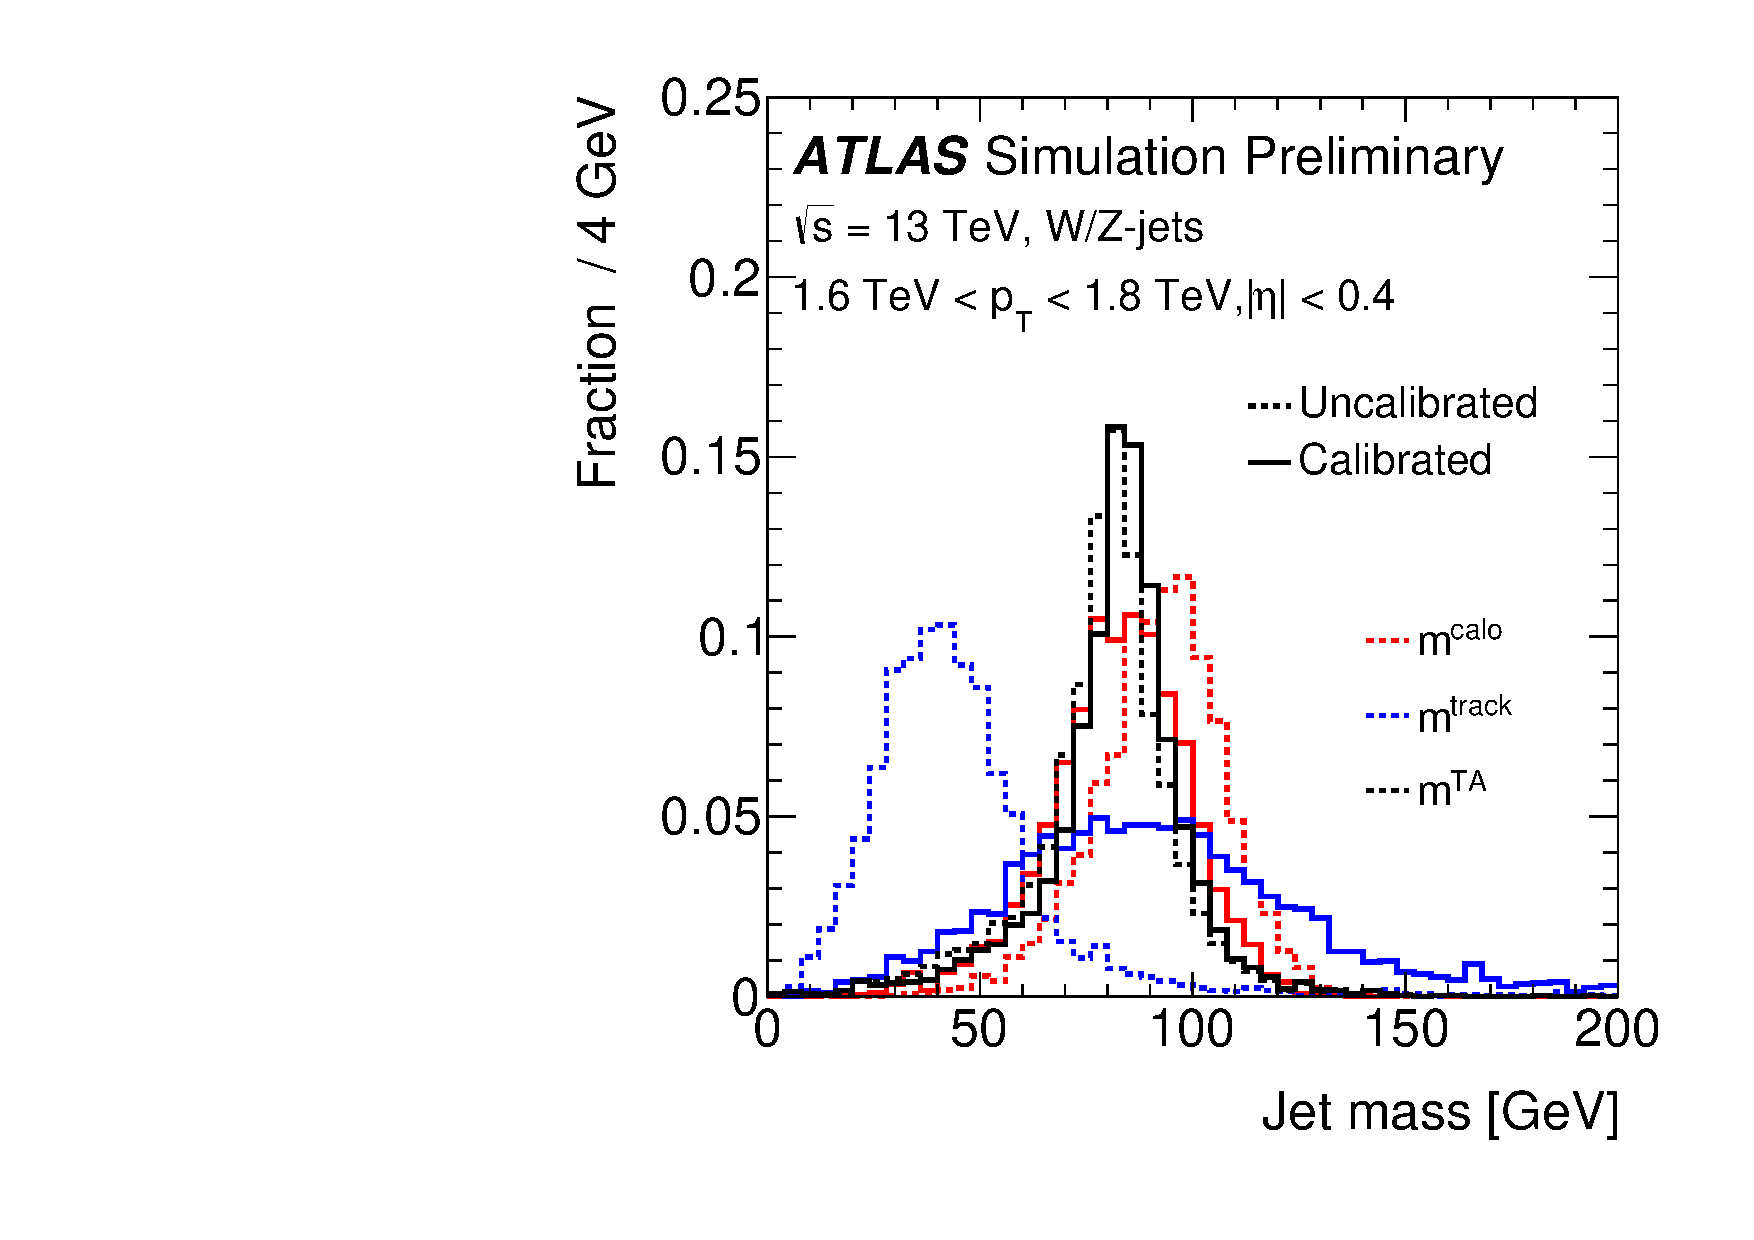
\includegraphics[width=\textwidth,angle=-90]{figures/object/Jet_mass}
        \caption{Uncalibrated (dashed line) and calibrated (solid line) jet mass distribution.}
        \label{fig:obj_jet_mass_dist}
    \end{subfigure}
    \quad
    \begin{subfigure}[b]{0.45\textwidth}
        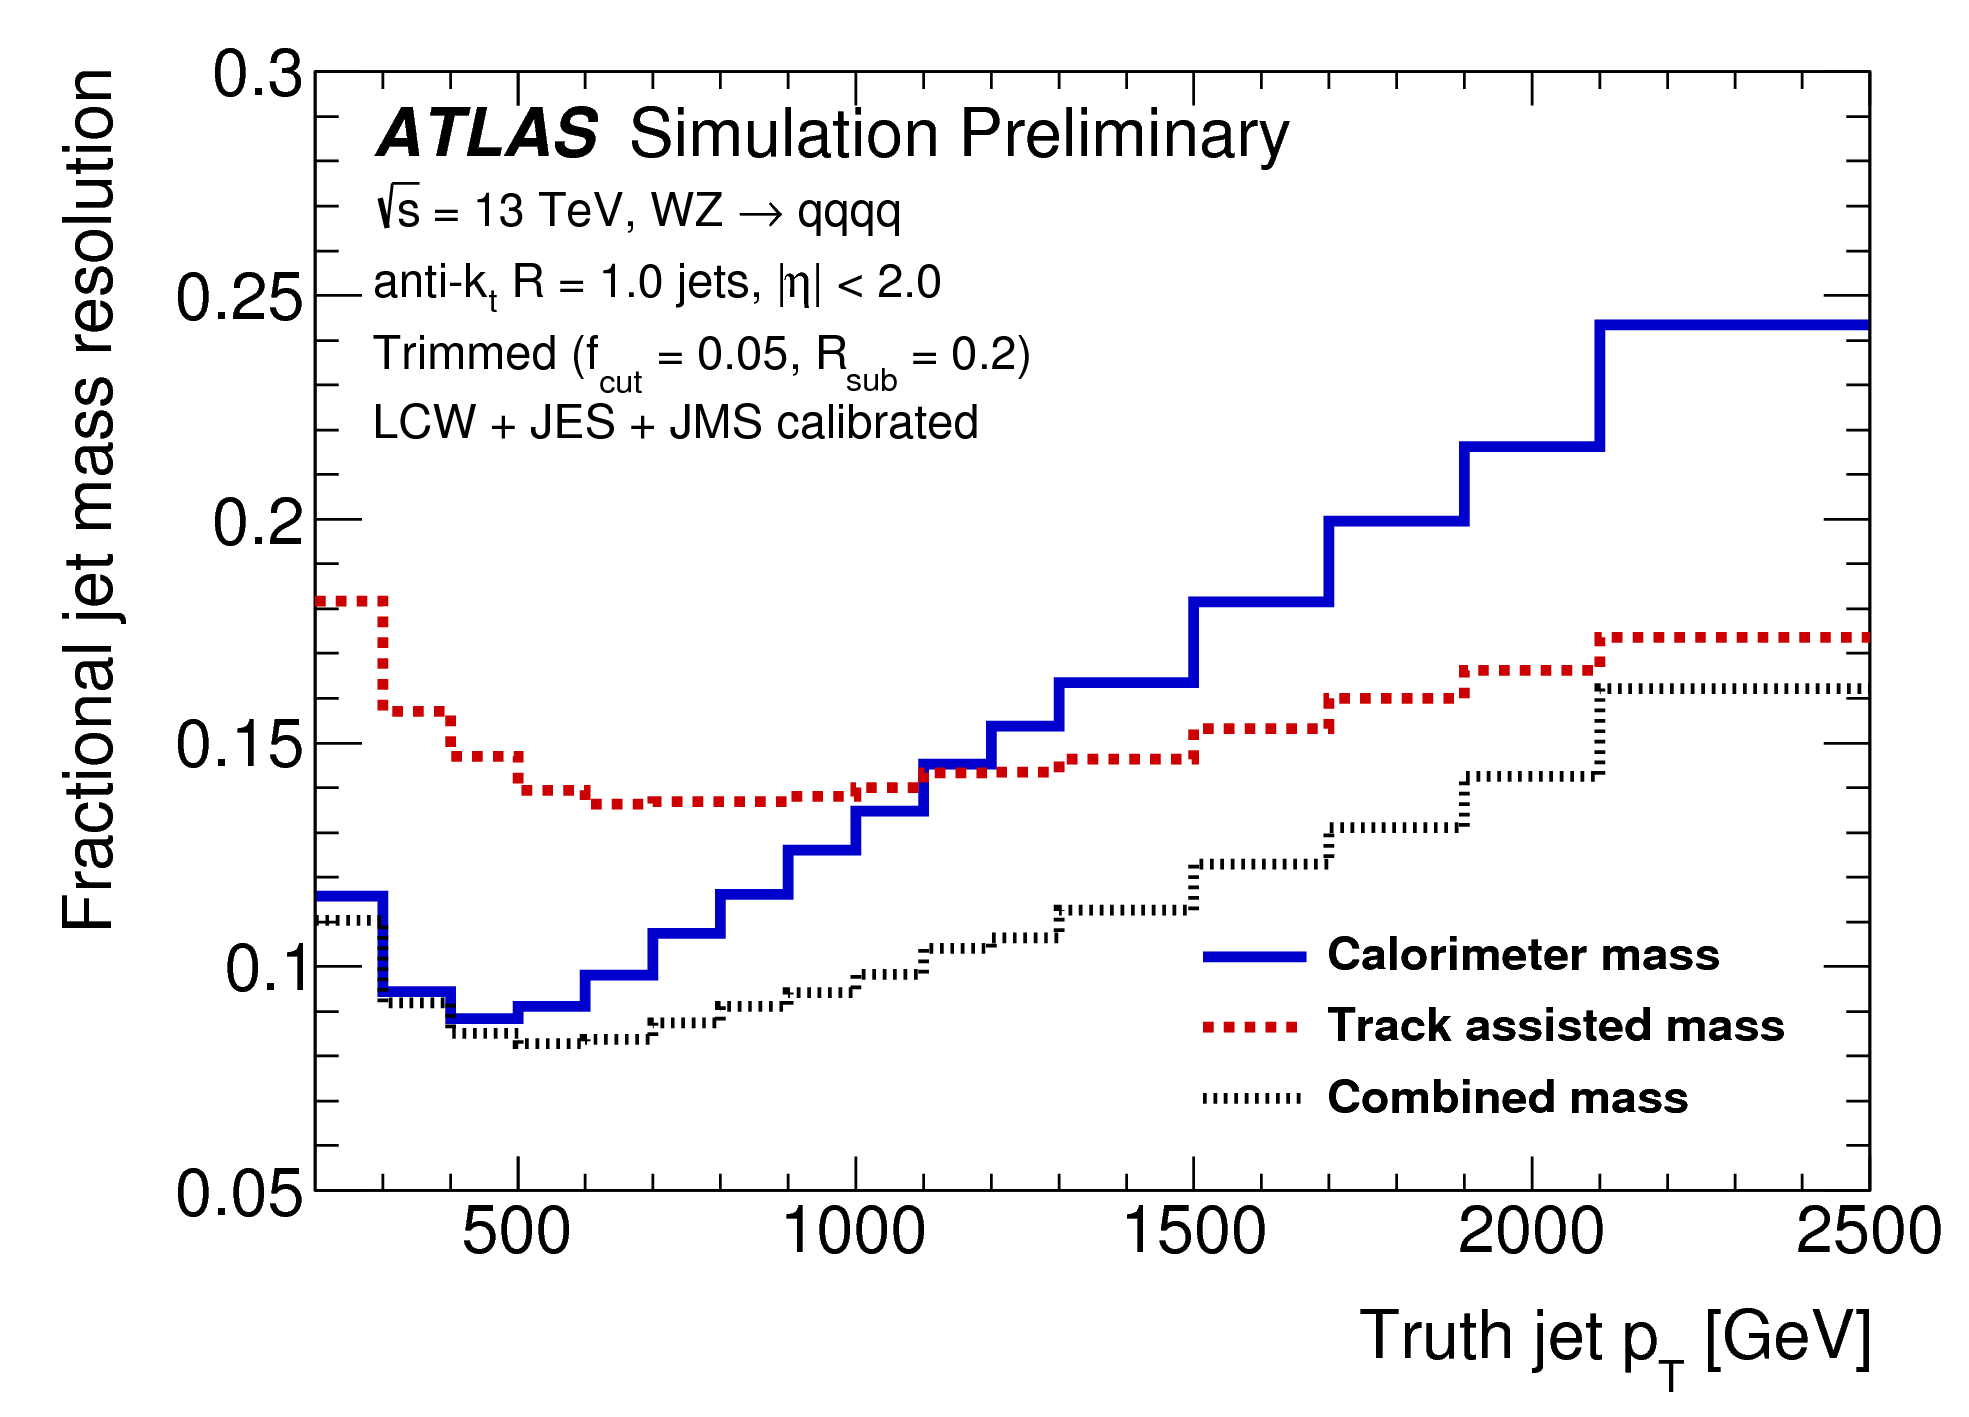
\includegraphics[width=\textwidth,angle=-90]{figures/object/Jet_mass_resolution}
        \caption{The factional jet mass resolution vs.  the truth jet mass transverse momentum.}
        \label{fig:obj_jet_mass_resolution}
    \end{subfigure}
   \caption{Uncalibrated (dashed line) and calibrated (solid line) reconstructed jet mass distribution ~\ref{fig:obj_jet_mass_dist}, and the jet mass resolution vs jet \pt ~\ref{fig:obj_jet_mass_resolution} for calorimeter-based jet mass, $m_{calo}$ (red), track-assisted jet mass $m_{TA}$ (black) and the invariant mass of four-vector sum of tracks associated to the large-radius calorimeter jet $m_{track}$ (blue) for W/Z-jets~\cite{ATLAS-CONF-2016-035}.}
  \label{fig:obj_jet_mass}
\end{figure}

\paragraph{}
The above two jet mass definitions are only weakly correlated with each other, so they can be linearly combined to the combined mass, $m^{comb}$, by weighting the components with $w$:
\begin{equation}
m^{comb} = w\cdot m^{calo}+(1-w)\cdot m^{TA}.
\end{equation}
where $w$ is determined for each large-\R jet from the resolution functions of the calibrated track and calo mass terms.
This results in a smaller mass resolution and better estimate of the median mass value than obtained using only calorimeter energy clusters, as shown in Figure~\ref{fig:obj_jet_mass}.

\subsection{Track Jets}
\label{obj:trackjet}
%The min $p_T$ is 400 MeV, and $|\eta| < 2.5$, and at least seven hits in the pixel or SCT. Total number of holes has to be less than two per track, and no more than one in the pixels. 
%$Z_{0}^{BL} \sin{\theta}$ is requred to be less than 3 mm.
\paragraph{}
Track jets are essentially clustered charged hadron tracks. 
They are reconstructed from ID tracks using the \akt~ algorithm with a fixed $R=0.2$. 
Once the track jet axis is determined, an extra step of track association is performed to select tracks with looser impact parameter requirements, in order to collect the tracks needed for effectively running the $b$-tagging algorithms.
Only track jets with at least two tracks are kept.
Track jets are also required to have $p_T > 10$ \GeV~ and $|\eta| < 2.5$, in order to suppress track jets from light flavors.

\paragraph{}
Track jets are associated to large-\R jets using Ghost-Association.
``Ghosts" are track jet 4-vectors, with each track jet's \pt~ set to an infinitesimal amount, essentially keeping only the direction of the 4-vector.
This ensures that Large-\R jets reconstruction is not altered by the ghosts when the calorimeter clusters plus ghosts are reclustered.
Reclustering is then performed using the \akt~ algorithm with $R=1.0$ .
The calorimeter jets after reclustering are identical to the parents of the trimmed jets used in this analysis, with the addition of the associated track jets retained as constituents.
In addition, the track jets corresponding to the ghosts that survive the trimming procedure (and thus are clustered into one of the surviving sub-jets) are the track jets ghost-associated to the trimmed jet.
The small radius parameter of the track-jets enables two nearby $b$-hadrons to be identified when their \DR~ separation is small, which is beneficial when reconstructing high-\pt~ Higgs boson candidates.

%%%%%%%%%%%%%%
\section{Flavor Tagging}
\label{sec:btag_70wp}
%b-tagging talk: https://cds.cern.ch/record/2280861/files/ATL-PHYS-SLIDE-2017-677.pdf
\paragraph{}
Some jets are formed from quarks with different flavors. 
Identifying the flavor of the jet parent quark is called flavor tagging. 
Jets originating from $b$-quarks are referred as $b$-jets, from $c$-quarks is referred as $c$-jets, and from other quarks other than the $t$-quark are referred as light jets.
$b$-tagging is particularly useful for this analysis, since there are four $b$-quarks in the final state.

\paragraph{}
$B$-hadrons have a lifetime $\tau$ on the order of $1.5 \times 10^{-12}$ seconds, which gives a flight path length $c\tau \sim 0.45\,\rm mm$~\cite{Pdg} without significant boost.
The mean flight path is $\beta\gamma c\tau$, where $\beta=\frac{v}{c}$ and $\gamma$ is the Lorenz factor.
With a higher boost, like $p_T = 50$ \GeV, the average transverse displacement is $3\rm mm$.
This results in a displaced decay vertex that can be identified in vertex reconstruction. 
This allows some $b$-jets to be distinguished from other flavors of jets.

\paragraph{}
ATLAS uses three different basic $b$-tagging algorithms, which provide complementary information:
\begin{itemize}
	\item Impact parameter based algorithm: it uses the signed transverse and longitudinal impact parameters $d_0$ and $z_0 sin\rm \theta$ of the tracks inside a jet to determine their consistency with the primary vertex. The algorithm uses simulated templates of $\frac{d_0}{\rm\sigma_{d_0}}$ and $\frac{\rm z_0 sin \theta}{\rm \sigma{\rm z_0 sin\theta}}$ for light, $c$, and $b$ jets and evaluates the likelihood of the jet coming from each of these types.
  %The sign is defined as positive if the track intersects the jet axis in front of the primary vertex, and as negative if the intersection lies behind the primary vertex.
  %The experimental resolution generates a random sign for the tracks originating from the primary vertex, while tracks from the b-/c-hadron decay normally have a positive sign.

	\item Secondary vertex (SV) reconstruction algorithm: it uses tracks inside the jet to look for vertices that are displaced from the primary vertex. The algorithm provides information on the invariant mass of tracks pointing to the displaced vertex, the number of two track vertices, and the angular separation between the jet axis and the PV $\to$ SV direction. The fraction of jets which have a reconstructed secondary vertex are shown in Figure~\ref{fig:obj_b_sv}. The increase of tracks from fragmentation in the high \pt~ region is the main reason for the performance degradation. The number of fake vertices is increasing with jet \pt~ in light jets, while the secondary vertex reconstruction efficiency for $b$/$c$-jets slightly decreases with jet \pt.

	\item Decay chain multi-vertex reconstruction algorithm, or JetFitter (JF): it reconstructs the full flight path of the $b$ by looking for multiple displaced vertices along the same direction. A Kalman filter is used to find common line for the $b$ and $c$ vertices, and hence the algorithm exploits the topology of the weak $b$/$c$-hadron decay chain. Leptonic decays of $b$/$c$ are not considered.
\end{itemize}
 
\begin{figure}[htbp!]
\centering
\captionsetup{justification=centering}
    \begin{subfigure}[b]{0.4\textwidth}
        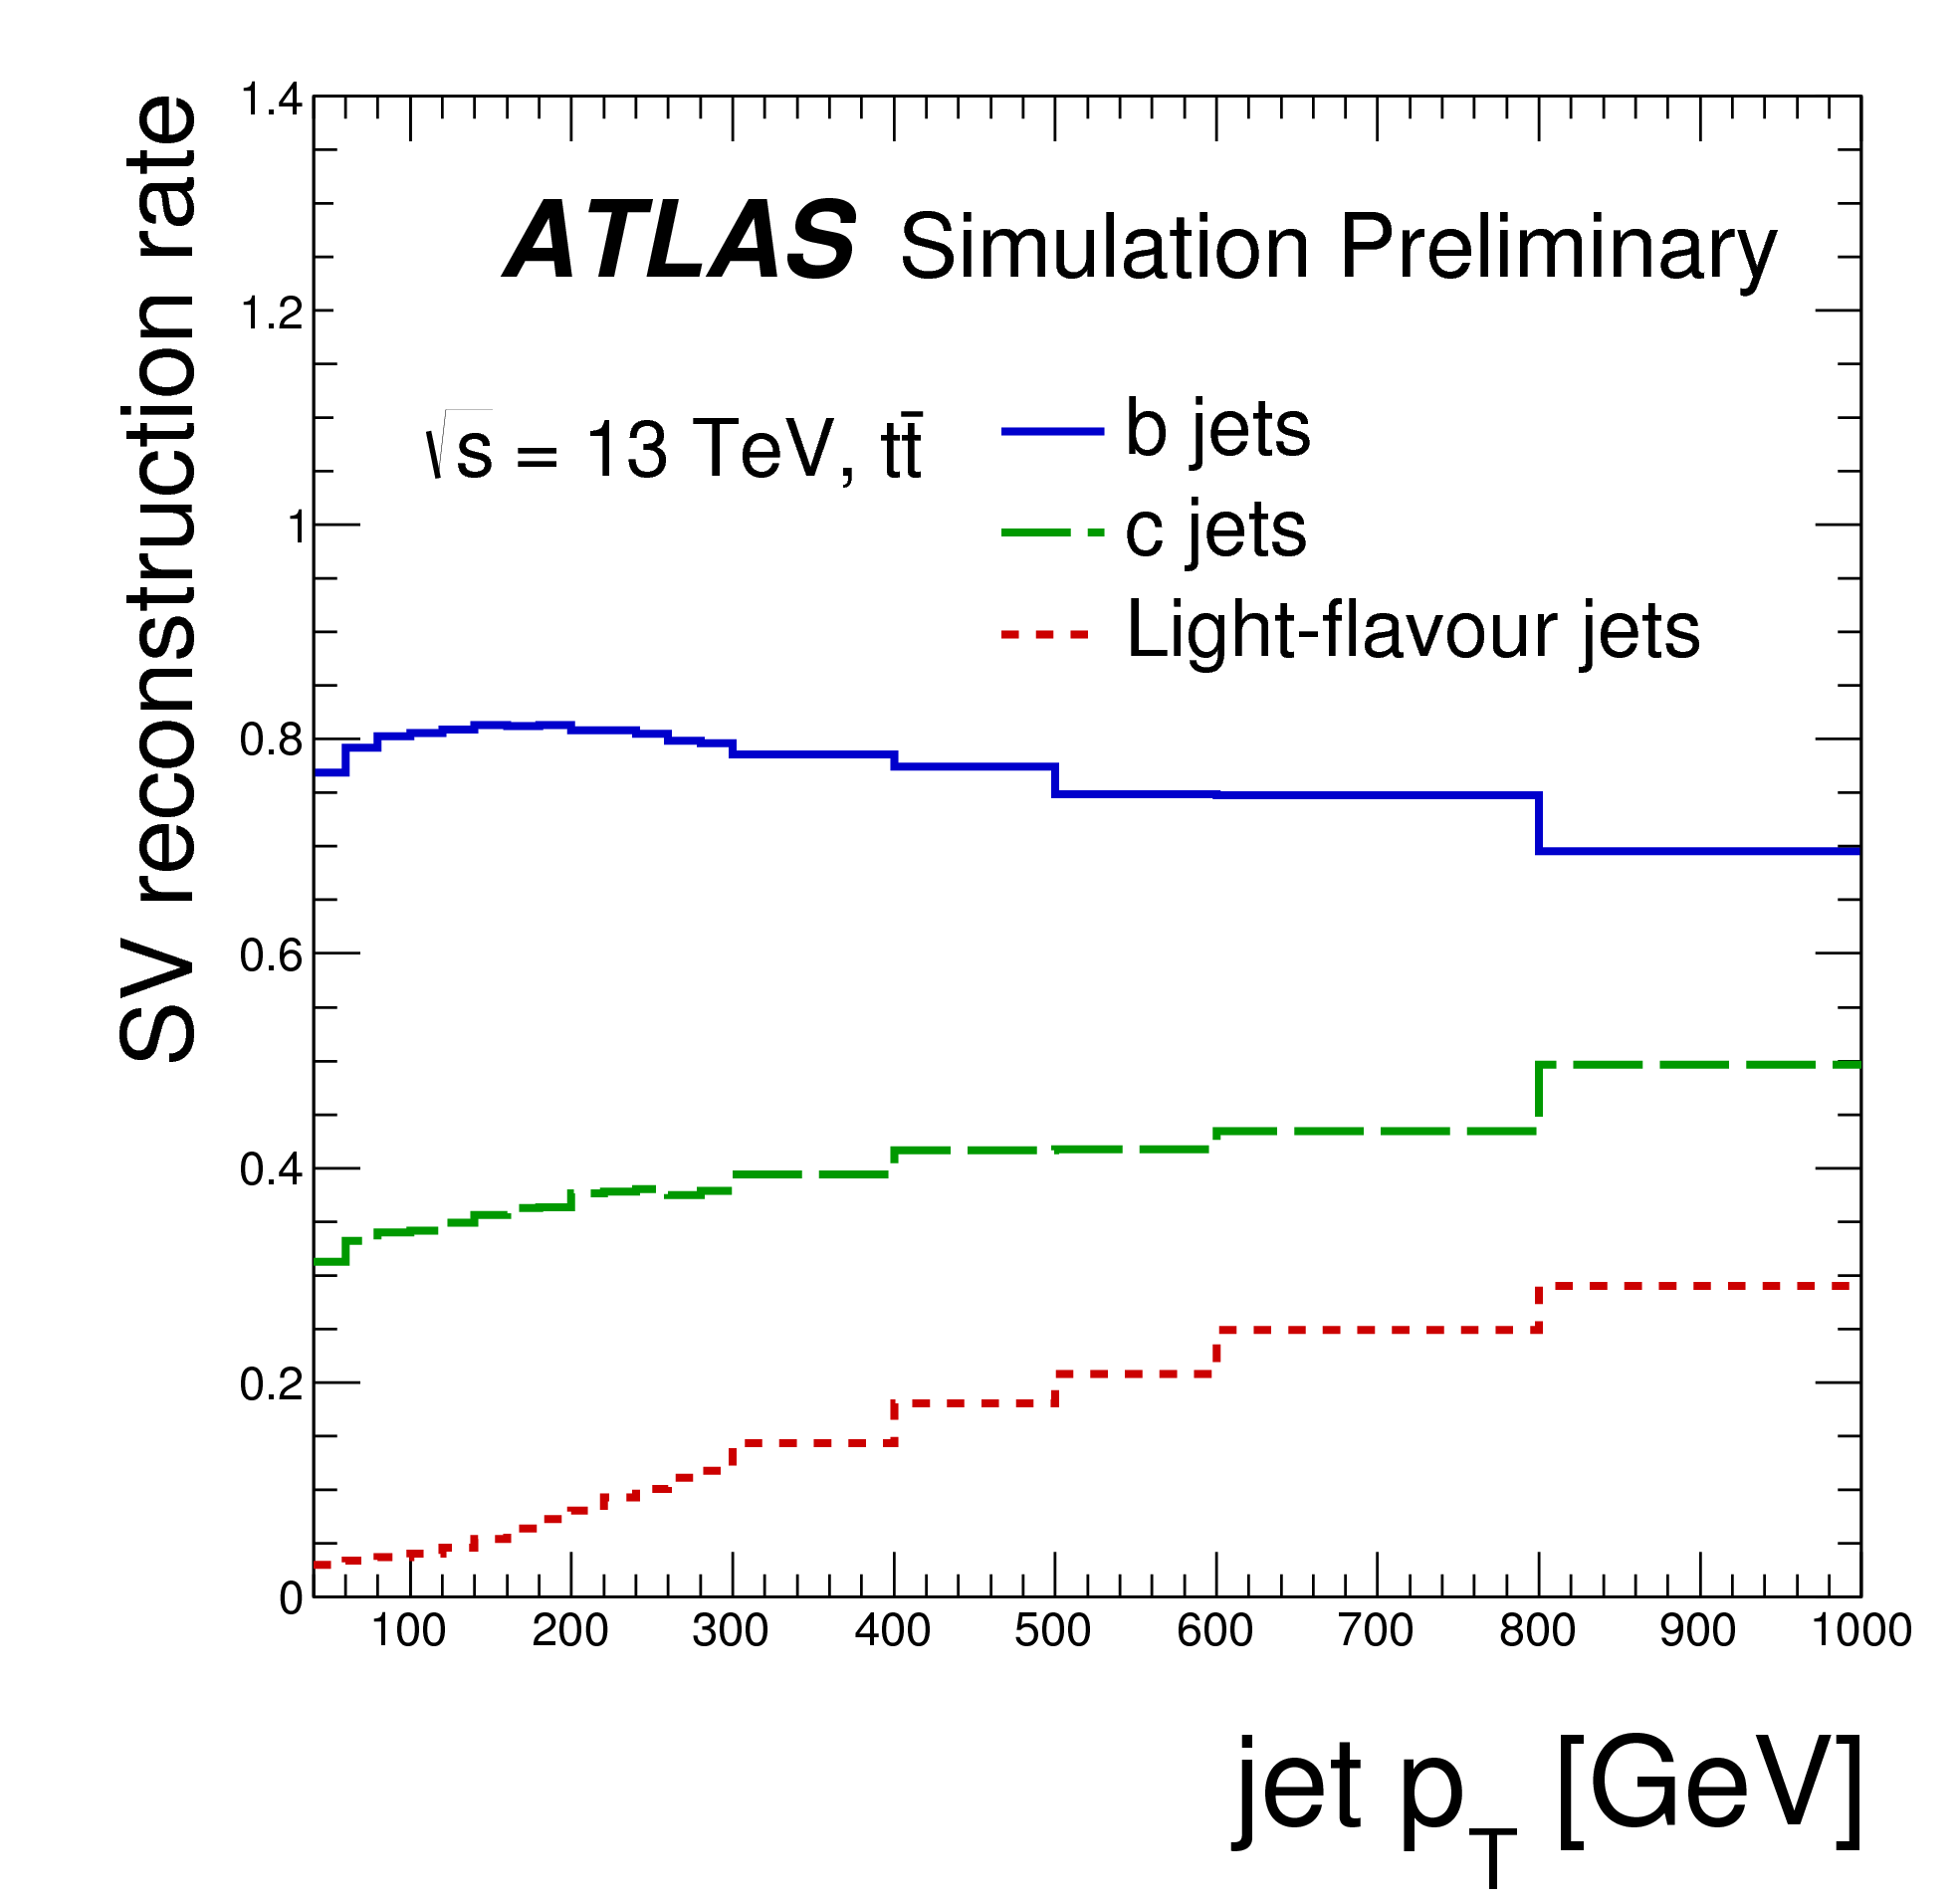
\includegraphics[width=\textwidth]{figures/object/b_sv}
        \caption{SV reconstruction rate vs. jet \pt.}
        \label{fig:obj_b_sv}
    \end{subfigure}
    \quad
    \begin{subfigure}[b]{0.43\textwidth}
        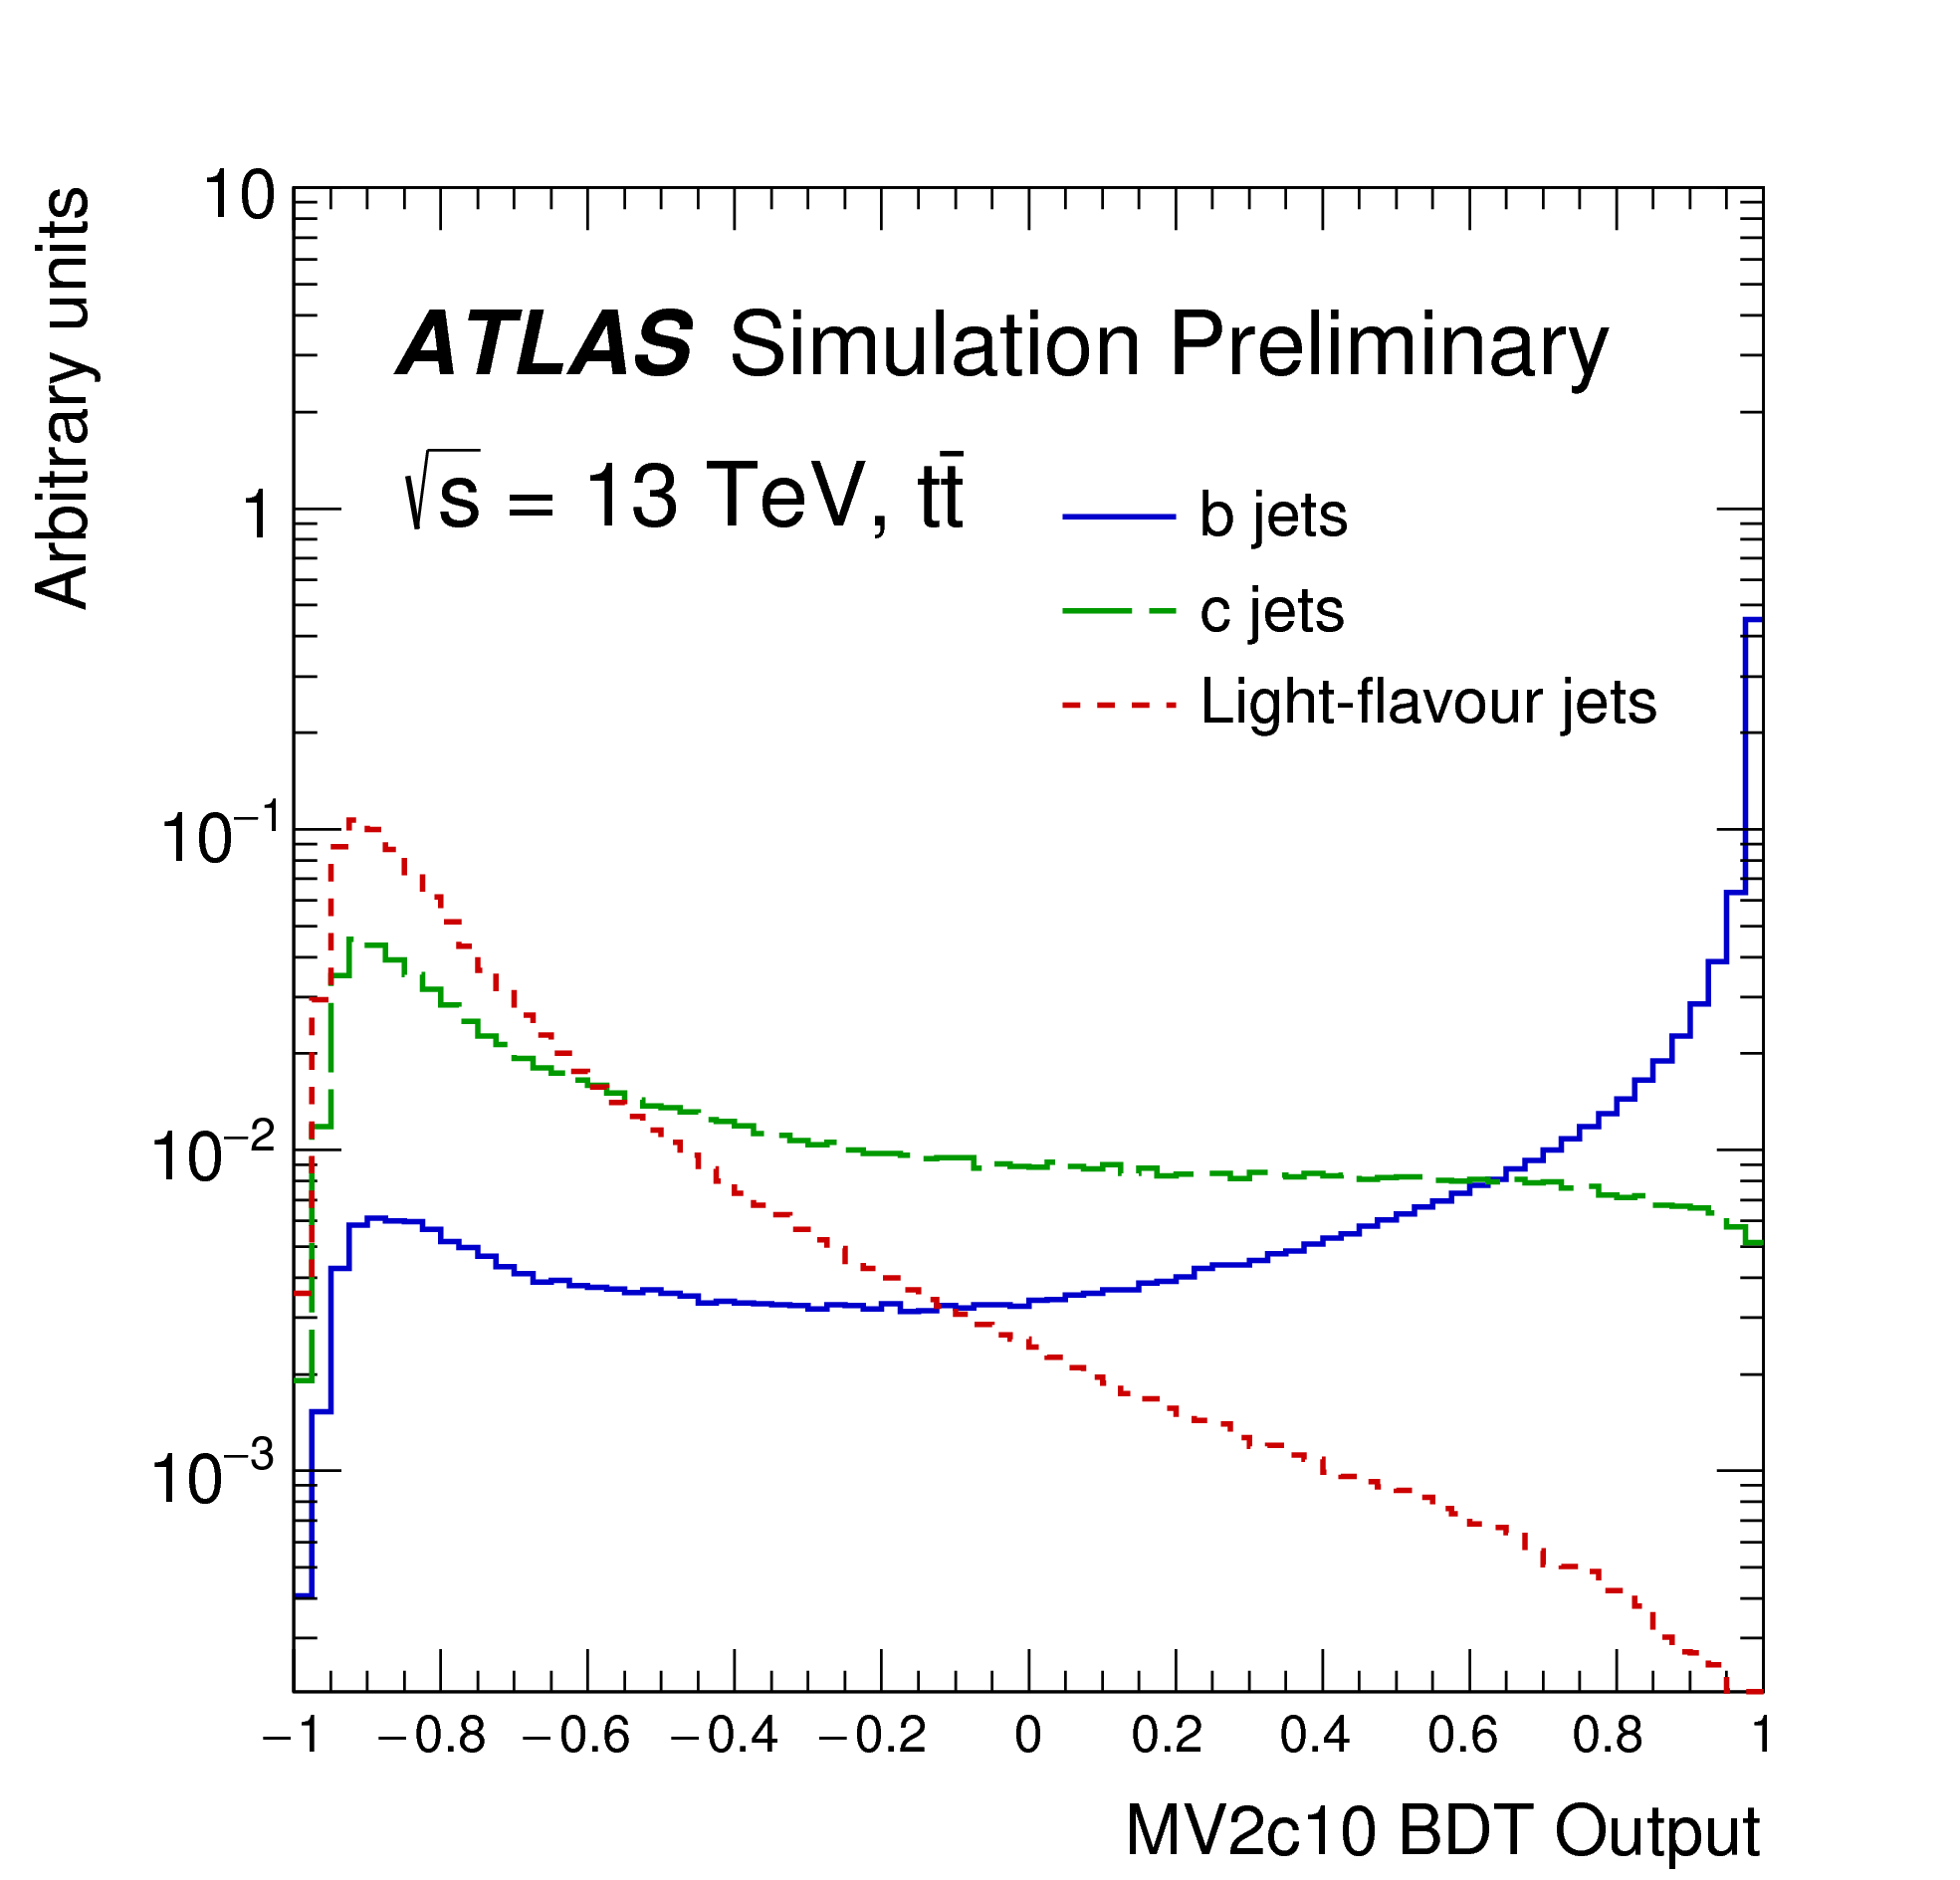
\includegraphics[width=\textwidth]{figures/object/b_mv2}
        \caption{MV2c10 BDT output for different jets.}
        \label{fig:obj_b_mv2}
    \end{subfigure}
\caption{Secondary vertex reconstruction rate and \emph{MV2c10} output for $b$-jets (solid blue), $c$-jets (dashed green) and light-jets (dotted red) evaluated with simulated \ttbar~ events.}
\label{fig:obj_btag}
\end{figure}

\paragraph{}
%%https://twiki.cern.ch/twiki/bin/view/AtlasProtected/BTaggingMV2
Jets containing $b$-hadrons are identified using a score value computed from a boosted decision tree(BDT) algorithm \emph{MV2c10}~\cite{btaggingRun2, Aad:2015ydr}, which makes use of observables provided by the three algorithms above.
A BDT consists of a forest of decision trees.
A number of individual decision trees are trained sequentially, with a boosting process in between each training. 
Boosting consists of adjusting the weights of individual events according to whether the previously trained tree classifies them correctly.
The \emph{MV2c10} algorithm is trained on a \ttbar~ sample, with $b$-jets as signal and a mixture of $93\%$ light-jets and $7\%$ c-jets as backgrounds. 
It is applied to a set of charged-particle tracks that satisfy quality and impact parameter criteria and are matched to each jet. 
The \emph{MV2c10} algorithm works on both small-\R jets or track jets.
%There are 3 taggers in MV2 family: \emph{MV2c00}, \emph{MV2c10}, \emph{MV2c20} depending on their charm composition in training. MV2c00$->0\%$ c-fraction in the training, MV2c10$->7\%$ c-fraction in the training and MV2c20$->15\%$ c-fraction in the training.

\paragraph{}
The $b$-tagging working point (wp) is a fixed cut on the \emph{MV2c10} value that lead to an efficiency of 70\% for $b$-jets with $p_T > 20$ \GeV~ when evaluated in a sample of simulated \ttbar~ events. 
This working point corresponds to a acceptance rate of light-jets or jets originating from gluons at $\frac{1}{380}$ for the jets with $R=0.4$ and $\frac{1}{120}$ for the track jets. The acceptance of jets from $c$-quarks is $\frac{1}{12}$ for the $R=0.4$ jets and $\frac{1}{7}$ for the track jets.

\begin{figure}[htbp!]
  \centering
  \captionsetup{justification=centering}
  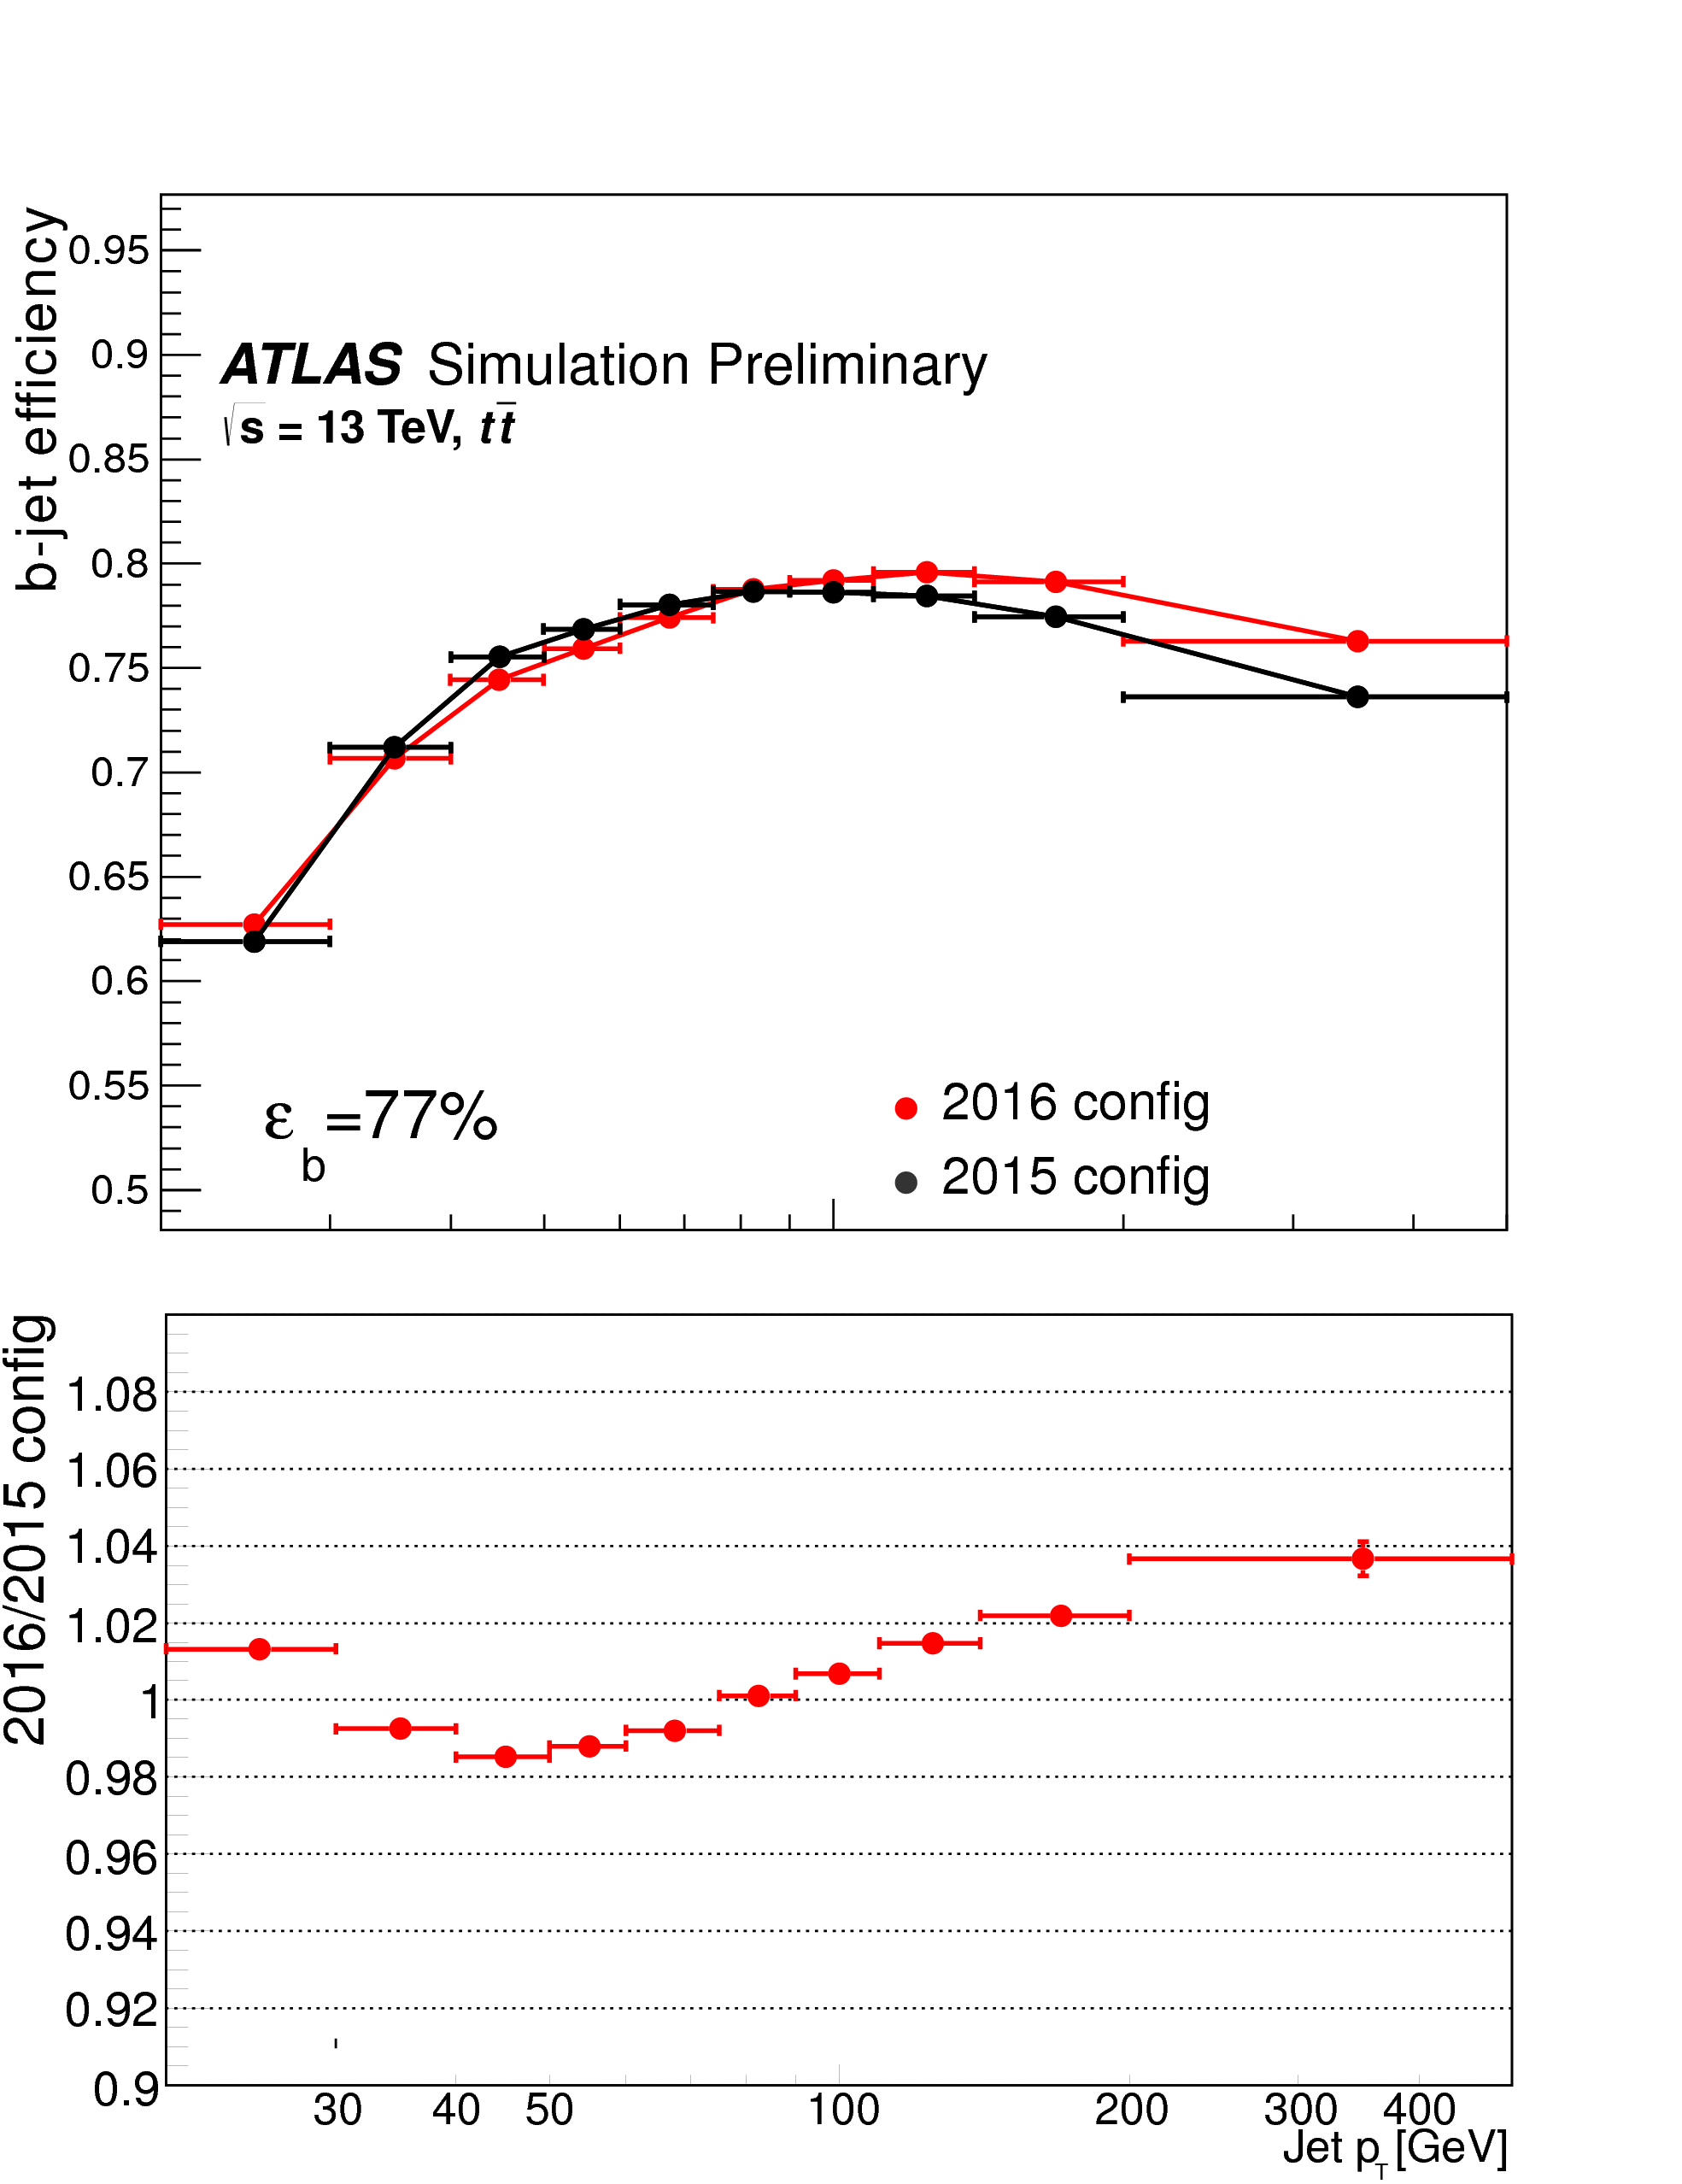
\includegraphics[width=0.5\textwidth]{figures/object/b_eff_pt}
   \caption{$b$-jet efficiency for the fixed cut working point with a $b$-jet efficiency of $77\%$ as a function of the jet \pt~ for the comparison between the \emph{MV2c10} $b$-tagging algorithm employed for the 2016 analyses (2016 config) and the previous version of the tagger, \emph{MV2c20} (2015 config), which has $15\%$ $c$-fraction in the training.}
  \label{fig:obj_b_eff}
\end{figure}

\paragraph{}
In this thesis, the track-jets have a wider \pt~ range, between $50-400$~\GeV, and the same working point leads to $b$-tagging efficiencies varying from $40\%$ at low \pt, to $80\%$ for \pt values of about $150$~\GeV, to $60\%$ at high \pt. 
This can be seen in Figure ~\ref{fig:obj_b_eff}, and the $b$-tagging efficiency varies from $60\%$ to $80\%$ for an average efficiency of $77\%$.
The increase of tracks from fragmentation in the high jet \pt~ region is the main reason for the performance degradation. 
As the jet \pt~ increases, the number of vertices from the random combination of high multiplicity tracks is increasing, while the secondary vertex reconstruction efficiency for $b$ and $c$-jets decreases with jet \pt.
This is shown in Figure ~\ref{fig:obj_btag_rej}, and the light-jet acceptance rate could range from $\frac{1}{120}$ to $\frac{1}{250}$.
This non-trivial jet \pt~ dependence of $b$-tagging performance is one of the major challenges of this analysis.

\begin{figure}[htbp!]
\centering
\captionsetup{justification=centering}
    \begin{subfigure}[b]{0.4\textwidth}
        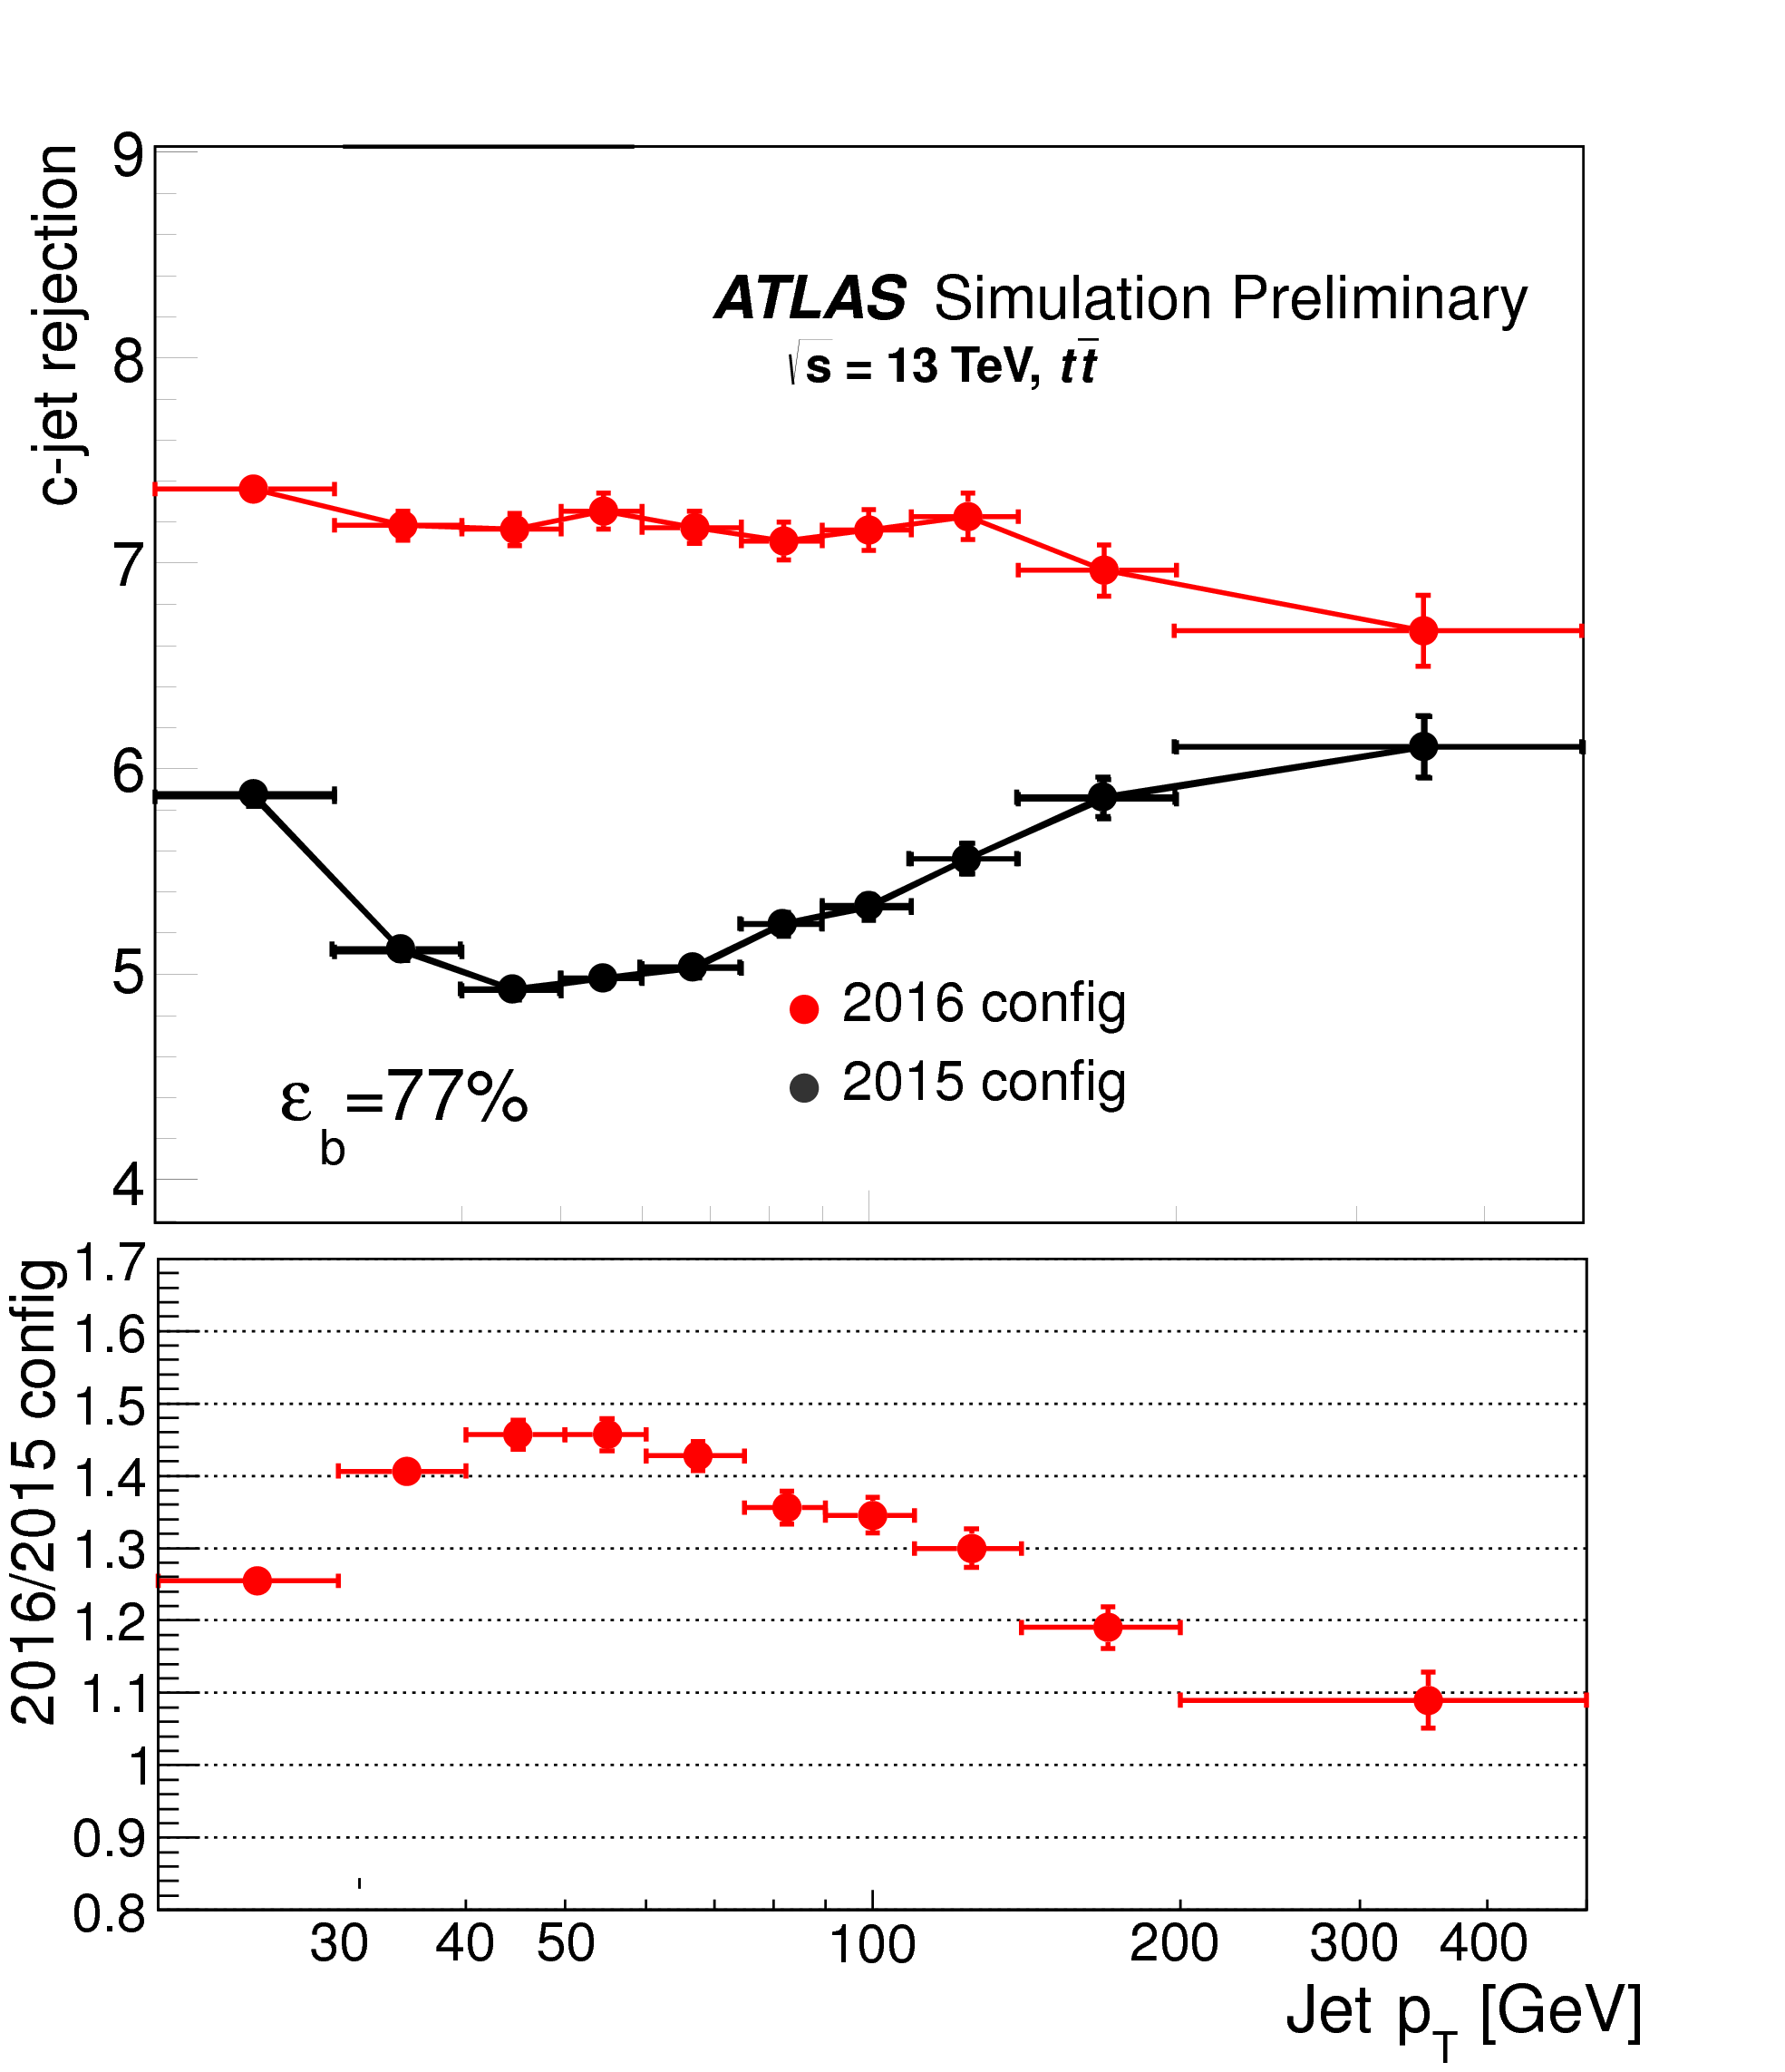
\includegraphics[width=\textwidth]{figures/object/c_rej_pt}
        \caption{$c$-jet rejection as a function of jet \pt.}
        \label{fig:obj_c_rej}
    \end{subfigure}
    \quad
    \begin{subfigure}[b]{0.4\textwidth}
        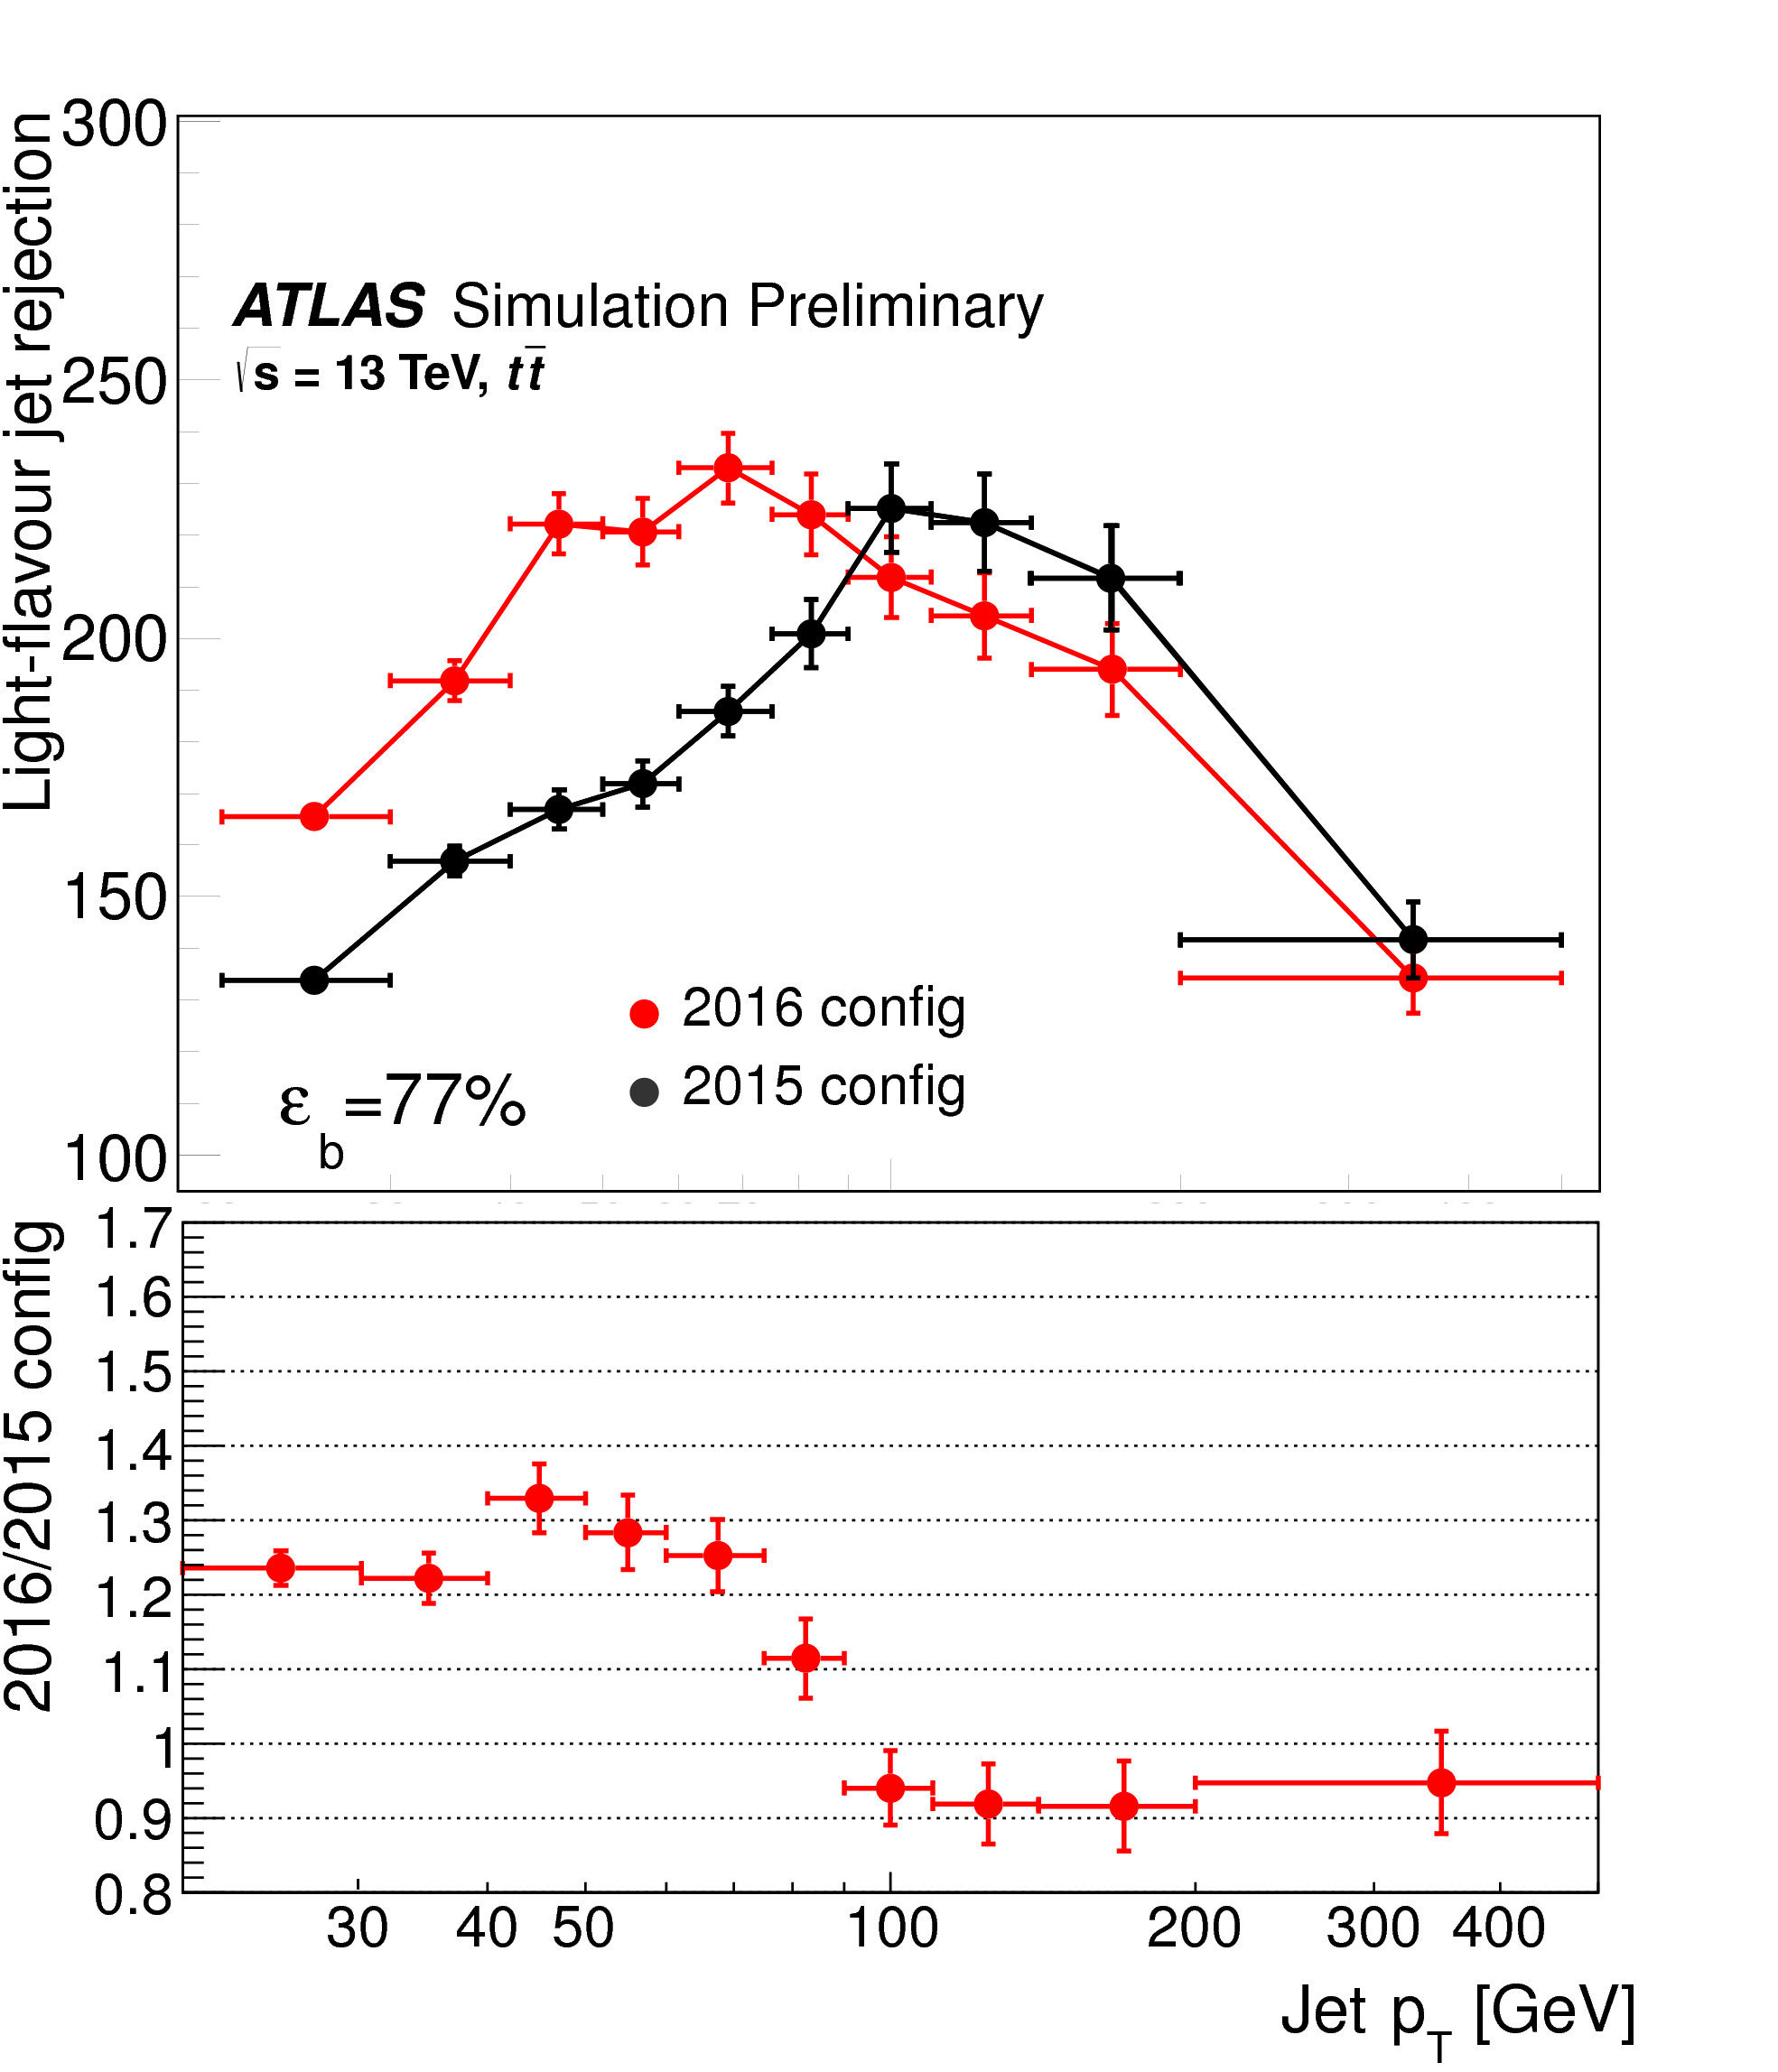
\includegraphics[width=\textwidth]{figures/object/light_rej_pt}
        \caption{Light jet rejection as a function of jet \pt.}
        \label{fig:obj_light_rej}
    \end{subfigure}
\caption{Light-flavour jet and $c$-jet rejection as a function of jet \pt~ for the previous (2015 config) \emph{MV2c20} and the current \emph{MV2c10} configuration (2016 config). A fixed cut at 77\% $b$-jet efficiency operating point is used ~\cite{btaggingRun2}.}
\label{fig:obj_btag_rej}
\end{figure}

%\paragraph{}
%$b$-tagging. see \href{https://cds.cern.ch/record/2160731/files/ATL-PHYS-PUB-2016-012.pdf}{2016 run2 note}. Recurrent Neural Network(RNN), which could explore more the correlation between different input parameters, especially the fragmentation of jets and the impact parameters, has shown improvements in $b$-tagging efficiency and is under investigation for future Multivariate Taggers, see \href{https://cds.cern.ch/record/2253371}{RNN note}. 

%Vertex reconstruction and resolution, can be seen in this \href{http://atlas.web.cern.ch/Atlas/GROUPS/PHYSICS/PUBNOTES/ATL-PHYS-PUB-2015-026/}{note}. Track resolution can be seen in this \href{https://cds.cern.ch/record/2110140/files/ATL-PHYS-PUB-2015-051.pdf}{note}. In Run2, the $d_0$ resolution is about 10 $\mu m$ and $z_0$ is about $50 \mu m$, both decreases as a function of track momentum.

%\paragraph{}
%See the reference \href{https://twiki.cern.ch/twiki/bin/viewauth/AtlasProtected/BTaggingPaperRecommendations}{here}. Operating points are defined by a single cut value on the discriminant output distribution and are chosen to provide a specific $b$-jet efficiency on an inclusive ttbar sample. (More information on the working points can be extracted from Table 2 and the related section in ATL-PHYS-PUB-2016-012).

\paragraph{}
%as can be seen in \href{https://indico.cern.ch/event/622490/contributions/2510894/attachments/1425202/2191220/ttbar_PDF_Calibration_MVA_Training_Approval_140317.pdf}{Likelihood talk} and \href{https://cds.cern.ch/record/1538335/files/ATL-COM-PHYS-2013-395.pdf}{Matrix method and Likelihood note} or a Tag-and-Probe using semi-leptonic $t\top{t}$ events.
Correction factors are applied to the simulated MC samples to compensate for differences between data and simulation in the b-tagging efficiency for $b$, $c$ and light-jets. The correction for $b$-jets is derived from \ttbar~ events with final states containing two leptons, and the corrections are consistent with unity with uncertainties at the level of a few percent over most of the jet \pt~ range.

%\paragraph{}
%Uncertainties on the correction factors for the $b$-tagging are applied to the simulated event samples by looking at dedicated \ttbar~ samples in data. An additional term is included to extrapolate the measured uncertainties to the high \pt~ region of interest. This term is calculated from simulated events by considering variations on the quantities affecting the b-tagging performance such as the impact parameter resolution, percentage of poorly measured tracks, description of the detector material, and track multiplicity per jet. The dominant effect on the uncertainty when extrapolating to high \pt~ r is related to the different tagging efficiency when smearing the track impact parameters based on the resolution measured in data and simulation.

%%%%%%%%%%%%%%
\section{Leptons}
%\paragraph{}
%Electron and photon identification is based on matching tracks to clusters in the ECAL and relying on the longitudinal and transverse shapes of the EM shower~\cite{ATLAS-CONF-2016-024}.
%Well-reconstructed ID tracks matched to EM clusters are classified as electron candidates, while EM clusters without matching tracks are classified as unconverted photon candidates. Clusters matched to a reconstructed conversion vertex or to pairs of tracks consistent with the conversion hypothesis are classified as converted photon candidates. 
%Electrons and photons are not used in this thesis.

%\paragraph{}
%Hadronic tau decays into a tau neutrino and one or three charged pions and up to two neutral pions~\cite{ATLAS-CONF-2017-029}. Hence tau reconstruction starts from jets, and the jets are matched to one or three associated tracks, with a total electric charge of $\pm 1$. A Boosted Decision Tree identification procedure, based on calorimetric shower shapes and tracking information is used to reject fakes. Hadronic taus are not used in this thesis.

%\paragraph{}
%Neutrinos are inferred from the missing transverse momentum (MET), or $E_T^{miss}$. Neutrinos do not interact with the ALTAS detector. Their presence can only be deduced from the conservation of transverse momentum in each collision, as the incoming protons have little net momentum in the transverse plane. MET is calculated as the negative vectorial sum of the \pt of all fully reconstructed and calibrated physics objects. This procedure includes a soft term, which is calculated using the ID tracks that originate from the primary vertex but are not associated with reconstructed objects. MET is not used in this thesis.

\paragraph{}
Muons are identified by matching ID tracks with reconstructed MS tracks~\cite{Aad:2016jkr}. 
For this thesis, muons must have $p_T > 4~\GeV$, $|\eta| < 2.5$ and to satisfy ``medium'' muon identification criteria~\cite{Aad:2016jkr}. 
Muons are used in this thesis, because $b$ hadrons decay to muons with $\sim 20\%$ probability. This is demonstrated in section~\ref{sec:obj-objectselection}.
%If a muon is within $\DR = 0.4$ (0.2) of a jet used for $b$-tagging in the resolved (boosted) analysis, their four-momentum is added to the calorimeter-based jet's four-momentum to partially account for the energy lost in semi-leptonic $b$-hadron decays.



%Although this work doesn't depend on specific boosted W/Z/H/Top taggers, many analysises adopt them and improve search sensitivities. For machine learning techiniques applied, see this \href{https://cds.cern.ch/record/2242830/files/ATL-COM-PHYS-2017-031.pdf}{W/Top tagger using BDT/DNN}

